\documentclass[a4paper,12pt]{scrartcl}
\usepackage{a4wide}
\usepackage[left=2cm, right=2cm, top=3cm]{geometry}
\usepackage{graphics}
\usepackage{mathtools}
\usepackage{amsmath, amssymb} 
\usepackage[utf8]{inputenc}
\usepackage[ngerman]{babel}
\usepackage{hyperref}
\usepackage{enumitem}
\usepackage{booktabs}
\usepackage{aligned-overset}  % Um bei Align die Gleichheitszeichen übereinander zu haben
\usepackage[version=4]{mhchem}
\usepackage{cancel}
\usepackage{wrapfig}
\usepackage{marvosym}
\usepackage[headsepline]{scrlayer-scrpage}
\usepackage{subcaption}
\usepackage{tabularx}
\usepackage{braket}
\usepackage{environ}
\usepackage{natbib}
\usepackage{tikzsymbols}
\usepackage[skins, xparse, breakable]{tcolorbox}
\usepackage{xcolor}
\usepackage{dsfont}
\usepackage{pdfpages} % https://www.namsu.de/Extra/pakete/Pdfpages.html
\allowdisplaybreaks  % Damit Align-Umgebungen umgebrochen werden können



% Set to 1 (only selection) or 0 (full script)
\newcounter{reduce_to_selection}
\setcounter{reduce_to_selection}{0}
% \setcounter{reduce_to_selection}{1}
% \includeonly{Woche07}


\newcommand{\Tipps}[2]{
    \ifnum\value{reduce_to_selection}=1 {
        \subsection{Tipps zu den Aufgaben von Blatt #1}
        \Disclaimer{}\\
        #2
    }
    \fi
}



\bibpunct{[}{]}{;}{a}{}{,}
\usepackage{scalerel}
\def\stretchint#1{\vcenter{\hbox{\stretchto[440]{\displaystyle\int}{#1}}}}
\def\bs{\mkern-12mu}
\pagestyle{scrheadings}
\clearpairofpagestyles


\numberwithin{equation}{section}
\let\oldsection\section  % Footnotecounter resetten
\renewcommand{\section}{\setcounter{footnote}{0}\oldsection}
\renewcommand{\thefootnote}{\Roman{footnote}}
\setlist[itemize]{topsep=1pt, itemsep=0pt, parsep=0.5pt}  % Itemize manipulieren
\setlist[enumerate]{topsep=1pt, itemsep=0pt, parsep=0.5pt}  % Itemize manipulieren


%%%%%%%%%%%%%%%%%%%%%%%%%%%%% Neue Umgebungen
\NewEnviron{Answer}
{%
\noindent
\rotatebox[origin=c]{180}{%
\noindent
\begin{minipage}[t]{\linewidth}
\BODY
\end{minipage}%
}%
}%

\newcommand{\C} {\mathbb{C}} 
\newcommand{\N} {\mathbb{N}} 
\newcommand{\Q} {\mathbb{Q}} 
\newcommand{\R} {\mathbb{R}}
\newcommand{\Z} {\mathbb{Z}}

\definecolor{mygreen}{RGB}{17,100,8}
\newtcolorbox[auto counter,number within=section]{Def}[2][]{%
breakable, enhanced, sharp corners, rounded corners=northwest, rounded corners=southeast, colback=blue!5!white,colframe=black!75!black,fonttitle=\bfseries,
title=Definition~\thetcbcounter: #2,#1}

\newtcolorbox[auto counter, number within=section]{Satz}[3][]{%
breakable, enhanced, sharp corners, rounded corners=southwest, rounded corners=northeast, colback=blue!5!white,colframe=red!75!black,fonttitle=\bfseries,
title=#2~\thetcbcounter: #3,#1}

\newtcolorbox[auto counter,number within=section]{Beispiel}[2][]{%
breakable, enhanced, colback=blue!5!white,colframe=blue!75!black, fonttitle=\bfseries,
title=Beispiel~\thetcbcounter: #2,#1}

\newtcolorbox[auto counter,number within=section]{Wiederholung}[2][]{%
breakable, enhanced, sharp corners, colback=green!5!white,colframe=mygreen!75!black, fonttitle=\bfseries,
title=Wiederholung~\thetcbcounter: #2,#1}

\makeatletter
\def\iddots{\mathinner{\mkern1mu\raise\p@
\vbox{\kern7\p@\hbox{.}}\mkern2mu
\raise4\p@\hbox{.}\mkern2mu\raise7\p@\hbox{.}\mkern1mu}}
\makeatother


\makeatletter
\newcommand{\tx}[1]{\text{#1}}
\newcommand{\Menge}[2]{\left\{#1\furdas#2\right\}}
\newcommand{\MengeDirekt}[1]{\left\{#1\right\}}
\newcommand{\diff}[2]{\frac{\text{d}#1}{\text{d}#2}}
\newcommand{\diffp}[2]{\frac{\partial#1}{\partial#2}}
\newcommand{\BiFo}[1]{\left\langle#1\right\rangle}
\newcommand{\Norm}[1]{\left|\left|#1\right|\right|}
\newcommand{\BiFoLeer}{\left\langle\cdot,\cdot\right\rangle}
\newcommand{\NormLeer}{\left|\left|\cdot\right|\right|}
\newcommand{\Spoiler}[1]{Hier werden wir nach Abgabe des Blattes den Lösungsweg skizzieren.}
\newcommand{\Matrix}[1]{\begin{pmatrix}#1\end{pmatrix}}
\newcommand{\MatrixAbs}[1]{\begin{vmatrix}#1\end{vmatrix}}
\newcommand{\MatrixInline}[1]{\left(\begin{smallmatrix}#1\end{smallmatrix}\right)}
\newcommand{\MatrixInvertieren}[2]{\left(\begin{matrix}#1\end{matrix}\,\left|\,\begin{matrix}#2\end{matrix}\right.\right)}
\newcommand{\Span}[2]{\text{span}\left\{#1\furdas#2\right\}}
\newcommand{\Spann}[1]{\text{span}\left\{#1\right\}}
\newcommand{\EinheitsN}{\mathds{1}_n}
\newcommand{\red}[1]{\textcolor{red}{\textbf{#1}}}
\newcommand{\blue}[1]{\textcolor{blue}{#1}}
\newcommand{\UausC}{Sei $U\subset\mathbb{C}$ offen}
\newcommand{\Res}{\text{Res}}
\newcommand{\qedsquare}{\hfill $\square$}
\newcommand{\qed}{\hfill \textbf{q.e.d.}}
\newcommand{\furdas}{\,|\,}
\newcommand{\mybox}[1]{\parbox[t]{8.5cm}{#1}}
\newcommand{\myboxU}[1]{\parbox[b]{8.5cm}{#1}}
\newcommand{\Zz}[1]{\textbf{Beh.}: \textbf{\textit{#1}}\\}
\newcommand{\Zb}[1]{\textbf{Bew.}: \blue{#1}\qedsquare}
\newcommand{\ZbOhne}[1]{\textbf{Bew.}: \blue{#1}}
\newcommand{\Skript}{\href{https://www.math.uni-hamburg.de/home/lentner/MfPh1/SkriptMfP1Lentner2020.pdf}{Skript}}
\newcommand{\Limes}[1]{\lim_{#1\rightarrow\infty}}
\newcommand{\LimesSum}[1]{\sum_{#1=0}^\infty}
\newcommand{\LimesSumOne}[1]{\sum_{#1=1}^\infty}
\newcommand{\LimesXiToX}{\lim_{\xi\to x}}
\newcommand{\SinusReihe}{\LimesSum{k}(-1)^k\frac{z^{2k+1}}{(2k+1)!}}
\newcommand{\KosinusReihe}{\LimesSum{k}(-1)^k\frac{z^{2k}}{(2k)!}}
\newcommand{\ExpReihe}[1]{\LimesSum{k}\frac{#1^{k}}{k!}}
\newcommand{\Cases}[1]{\begin{cases}#1\end{cases}}
\newcommand{\Id}{\text{Id}}
\newcommand{\BracedIn}[1]{\left({#1}\right)}
\newcommand{\BracedInSqr}[1]{\left[{#1}\right]}
\newcommand{\Abs}[1]{\left|{#1}\right|}
\newcommand{\artanh}{\text{artanh}}
\newcommand{\arsinh}{\text{arsinh}}
\newcommand{\arcosh}{\text{arcosh}}
\newcommand{\Disclaimer}{\textcolor{blue}{
$\left[\,\text{\parbox{0.95\textwidth}{\vspace{0.1cm}\textit{\textbf{Hinweis:}\\
Da wir euch offiziell nichts vorsagen sollen (was ja auch sinnvoll ist), sind die Tipps sehr allgemein gehalten. Hoffentlich helfen sie euch trotzdem, Ansätze zu finden, falls ihr mal nicht weiter kommt.\\
Bei konkreten Fragen helfen wir gerne persönlich.\vspace{0.1cm}}}}\,\right]$
}}
\newcommand{\Einleitung}[1]{\subsection*{Ausblick}
    \textcolor{blue}{\textit{#1}}}
\newcommand{\IV}{\text{IV}}
\newcommand{\im}{\text{im}}
\newcommand{\Abb}{\text{Abb}}
\newcommand{\Bij}{\text{Bij}}
\newcommand{\I}{\text{I}}
\newcommand{\II}{\text{II}}
\newcommand{\III}{\text{III}}
\newcommand{\card}{\text{card}}
\newcommand{\diag}{\text{diag}}
\newcommand{\grad}{\text{grad}}
\newcommand{\Hess}{\text{Hess}}
\newcommand{\rot}{\text{rot}}
\newcommand{\divv}{\text{div}}
\newcommand{\Diff}{\text{Diff}}
\newcommand{\Met}{\text{Mat}}
\newcommand{\Tr}{\text{Tr}}
\newcommand{\rg}{\text{rg}}
\newcommand{\End}{\text{End}}
\newcommand{\Aut}{\text{Aut}}
\newcommand{\GL}{\text{GL}}
\newcommand{\SL}{\text{SL}}
\newcommand{\ad}{\text{ad}}
\newcommand{\sgn}{\text{sgn}}
\makeatother
%%%%%%%%%%%%%%%%%%%%%%%%%%%%%%
\let\oldhref\href
\renewcommand{\href}[2]{\oldhref{#1}{\underline{\bfseries#2}}}
\renewcommand{\Re}{\text{Re}}
\renewcommand{\Im}{\text{Im}}
\newcommand{\rvec}{{\Vec{r}}}
\newcommand{\uvec}{{\Vec{u}}}
\newcommand{\pvec}{{\Vec{p}}}
\newcommand{\qvec}{{\Vec{q}}}
\newcommand{\jvec}{{\Vec{j}}}
\newcommand{\vvec}{{\Vec{v}}}
\newcommand{\fvec}{{\Vec{f}}}
\newcommand{\gvec}{{\Vec{g}}}
\newcommand{\hvec}{{\Vec{h}}}
\newcommand{\lvec}{{\Vec{l}}}
\newcommand{\evec}{{\Vec{e}}}
\newcommand{\yvec}{{\Vec{y}}}
\newcommand{\bvec}{{\Vec{b}}}
\newcommand{\cvec}{{\Vec{c}}}
\newcommand{\nablavec}{{\Vec{\nabla}}}
\newcommand{\alphavec}{{\Vec{\alpha}}}
\newcommand{\psivec}{{\Vec{\psi}}}
\newcommand{\varphivec}{{\Vec{\varphi}}}
\newcommand{\xivec}{{\Vec{\xi}}}
\newcommand{\avec}{{\Vec{a}}}
\newcommand{\svec}{{\Vec{s}}}
\newcommand{\nvec}{{\Vec{n}}}
\newcommand{\xvec}{{\Vec{x}}}
\newcommand{\Fvec}{{\Vec{F}}}
\newcommand{\Gvec}{{\Vec{G}}}
\newcommand{\wvec}{{\Vec{w}}}
\newcommand{\zvec}{{\Vec{z}}}
\newcommand{\dvec}{{\Vec{d}}}
\newcommand{\graph}{\text{graph}}
\newcommand{\Nullvec}{{\Vec{0}}}
\renewcommand{\Vec}[1]{{\text{\boldmath${#1}$}}}%\overset{_\rightharpoonup}

% \renewcommand{\Vec}[1]{{\mathbf{#1}}}%\overset{_\rightharpoonup}
\setlength{\parindent}{0pt}		 %Verhindert den automatischen Erstzeileneinzug



%%%%%%%%%%% Titel, Profs, Zeitraum etc.
\newcommand{\titel}{Notizen zur Vorlesung\\
\textit{Mathematik III für Studierende der Computing in Science, Geophysik/ Ozeanographie, Meteorologie und Physik}\\
WiSe 2022/23
}
\newcommand{\Kurztitel}{MfP3-Notizen}
\newcommand{\Zeitraum}{WiSe 2022/23}
\newcommand{\Profs}{Vorlesung von Dr. \textsf{Ralf Holtkamp}}
%%%%%%%%%%%
\automark{section}
\ihead{\textit{\Kurztitel}}
\chead{\emph{\headmark}}
\ohead{\Zeitraum}
\cfoot{\pagemark}

\title{\titel}
\date{\Zeitraum}



\begin{document}


\setlength{\abovedisplayskip}{3pt}
\setlength{\belowdisplayskip}{3pt}
\setlength{\abovedisplayshortskip}{3pt}
\setlength{\belowdisplayshortskip}{3pt}

	\thispagestyle{empty}
	\rule{\linewidth}{1pt}
	
	\vspace{6pt}				%Die Leerzeilen müssen tatsächlich da sein, sonst funktioniert das nicht
	
	\begin{minipage}{0.6\textwidth}
		\begin{flushleft} 
		\Profs
		\end{flushleft}
	\end{minipage}
	\begin{minipage}{0.39\textwidth}
		\begin{flushright}
			Universität Hamburg
		\end{flushright}
	\end{minipage}

	\rule{\linewidth}{1pt}\\
	\begin{center}
		\Large{\textsf{\titel}}\\
		\small\textsf{Version vom \today}
\vspace{8pt}
\end{center}


\begin{figure}[htbp]
    \centering
    
\includegraphics[width=.55\textwidth]{Dateien/3D_Analysis.jpg}\\
    Analysis, aber diesmal in 3D!\\
\end{figure}
\vfill
Grüßt euch, dies sind die Community MfP3-Notizen. \\

Sissi und ich erstellen sie als Nachbereitung der Vorlesung und sie dienen als eine schnelle Quelle von Definitionen und einfachen Beispielen (um sich einen Überblick zu verschaffen), wichtigen Bemerkungen aus den Übungen, sowohl als Klausurnotizen. Wir bewundern die informellen Notizen zum MfP1- und MfP2-Tutorium von Robin Löwenberg und Fabian Balzer und haben uns entschloßen mit dem gleichen Stil weiterzumachen, da es keine MfP3 und MfP4 Tutoriumnotizen mehr gibt. Die Templates wurden von Fabian erstellt und sind auf seiner Github-Seite verfügbar:  \url{https://github.com/Fabian-Balzer/MfP2-Notizen}. Zusätzlich benutzen wir das Lehrwerk Mathematik von Tilo Arens als eine Quelle von guten Beispielen. Das Buch können wir jedem empfehlen, der auch Giancoli mag und am besten an Beispielen lernt. Bei Anmerkungen oder Fragen schreibt uns einfach auf Whatsapp, Discord oder GitHub an. \\ 

Möge die Macht der endlosen zerbrochenen Kreiden mit euch sein :)

\cfoot{\pagemark}



\ifnum\value{reduce_to_selection}=0 {
    \tableofcontents
}\fi


%%%%%%%%%%%%%%%%%%%%%%%%%%%%%%%%%%%%%%%%%%%%%%%%%%%%%%%%%%%%%%%%%
\newpage
\section[Wiederholung]{Riemann-Integrale und Untermannigfaltigkeiten}
\subsection{Riemann-Integrale}\label{ssec:Riemann-Integrale}
\begin{Def}
{Ober- und Unterintegral}
Sei $f:[a,b]\rightarrow \R$ eine beschränkte Funktion. Das \red{Oberintegral} von $f$ ist die Zahl
$$\int_a^{*b}f(x)dx=\inf \{ \int_a^b \varphi(x)dx | \varphi \text{ Treppenfunktion mit } \varphi\geq f \} $$
Das \red{Unterintegral} von $f$ ist die Zahl
$$\int_{*a}^{b}f(x)dx=\sup \{ \int_a^b \varphi(x)dx | \varphi \text{ Treppenfunktion mit } \varphi\leq f \} $$
\end{Def}

\begin{Def}
{Riemann-integrierbare Funktion}
Eine beschränkte Funktion $f:[a,b]\rightarrow \R$ heißt \red{Riemann-integrierbar}, wenn $$\int_a^{*b}f(x)dx=\int_{*a}^bf(x)dx$$
\end{Def}
Ebenso ist es in der Analysis nützlich den Begriff des uneigentlichen Integrals zu verstehen, wenn der Definitionsbereich unbeschränkt ist.
\begin{Def}
{Uneigentliches Integral}
Sei $f:(a,b]\rightarrow \R$ nicht unbedingt beschränkt, aber für jedes Teilinterval $[\alpha, b] \in (a,b]$ integrierbar. Falls dann der Grenzwert
$$\lim_{\epsilon\rightarrow a}\int_\epsilon^{b} f(x)dx$$ existiert, so nennen wir $f$ über das Intervall $(a,b]$ \red{uneigentlich integrierbar}.
\end{Def}
\begin{Beispiel}
{Uneigentliches Integral}
Betrachten wir $\int_0^1 \frac{1}{\sqrt{x}}dx$. Dieses Integral kann als uneigentliches integral sinnvoll definiert werden:
$$\lim_{\epsilon\rightarrow 0}\int_\epsilon^1 \frac{1}{\sqrt{x}} dx =\lim_{\epsilon\rightarrow 0} [2\sqrt{x}]_\epsilon^1=\lim_{\epsilon\rightarrow 0}2\sqrt{1}-2\sqrt{\epsilon}=2$$
\end{Beispiel}
Die Gamma-Funktion $\Gamma(s)=\int_0^\infty t^{s-1}e^{-t}dt$ ist sehr nützlich, denn es gilt $\Gamma(s+1)=s\Gamma(s)$, also ist die Funktion perfekt dazu geeignet, um die Fakultät zu berechnen: $\Gamma(n)=(n-1)!$. Zusätzlich gilt $\Gamma(\frac{1}{2})=\sqrt{\pi}$.

\subsection{Topologie und Untermannigfaltigkeiten}\label{ssec:Topologie}
Gewisse topologische Begriffe sind auch im MfP3 sehr wichtig.
\begin{Def}
{Offene Kugel}
Die Teilmenge $\boxed{B_r(\xvec):=\Menge{\yvec\in X}{d(\xvec,\yvec)<r}\subseteq X}$ eines metrischen Raumes $(X,d)$ mit Abstandsfunktion $d$ heißt \red{offene Kugel} mit Mittelpunkt $\xvec$ und Radius $r$.
\end{Def}
\begin{Def}
{Inneres}
Für eine Teilmenge $A\subseteq X$ nennen wir die Vereinigung aller offenen Teilmengen das \red{Innere $\mathring{A}$} von $A$, also $\mathring{A}=\bigcup_{B\subseteq A}B$.
\end{Def}

\begin{Def}
{Abschluss}
Für eine Teilmenge $A\subseteq X$ nennen wir den Durchschnitt aller abgeschlossenen Mengen, die $A$ enthalten, den \red{Abschluss $\Bar{A}$} von $A$, also $\Bar{A}=\bigcap_{B\supset A, B\tx{ abgeschl.}}B$.
\end{Def}
\begin{Def}
{Rand}
Die Differenz aus diesen beiden Mengen ist dann der \red{Rand $\partial A$} von $A$, also $\partial A=\Bar{A}\setminus \mathring{A}$.
\end{Def}
\begin{Def}
{Kompaktheit}
Falls wir zu \underline{jeder} offenen Überdeckung $(U_i)_{i\in I}$ von $A\subseteq X$ eine endliche Teilüberdeckung, d.h. eine Einschränkung der Indexmenge $I$ auf eine endliche Menge $J\subseteq I$ finden, sodass $(U_i)_{i\in J}$ immer noch eine offene Überdeckung von $A$ ist, so nennen wir $A\subseteq X$ \red{kompakt}.
\end{Def}
\begin{Satz}
{Folgerung}{Kompakte Teilmengen sind abgeschlossen und beschränkt}
Jede kompakte Teilmenge $A\subseteq X$ eines metr. Raumes ist \underline{abgeschlossen}, \underline{vollständig} und \underline{beschränkt}.
\end{Satz}
\begin{Def}{Separable Räume und Dichtigkeit}
    Die Metrik $(X,d)$ heißt separabel, falls es eine abzählbare dichte Teilmenge in $X$ gibt. \\
    Eine Teilmenge $Y\subseteq X$ heißt dicht in $X$, wenn $\overline{Y}=X$.
    $$\forall \epsilon>0 \forall x\in X \exists y\in Y: d(x,y) <\epsilon$$
\end{Def}
Jetzt gehen wir über zu Untermannigfaltigkeiten und schließen die Wiederholung mit allgemeinen Mannigfaltigkeiten ab.
\begin{Def}
{Immersion}
Ist $\rg(f)=m\,\forall \pvec\in U$, d. h. die Abbildung hat den konstanten Rang der Dimension des \underline{Urbildraums}, so sagen wir, dass $f$ eine \red{Immersion} ist.\\
Das Differential $df:U\to\mathbb{R}^n$ ist dann injektiv. 
\end{Def}
Die $C^k(I,\R)$ ist eine $k$-fach stetig differenzierbare Funktion.
\begin{Def}
{$C^k$-Diffeomorphismen}
$C^k$-Abbildungen $f:U\to V$, die bijektiv sind und deren Umkehrabbildungen auch $C^k$ sind, nennen wir \red{$C^k$-Diffeomorphismen}.
\end{Def}
\begin{Beispiel}
{Bekannter Diffeomorphismus}
Die Abbildung $f:\mathbb{R}\to\mathbb{R}_+\setminus\MengeDirekt{0},\,f(x)=e^x$ ist mit $f^{-1}:\mathbb{R}_+\setminus\MengeDirekt{0}\to\mathbb{R},\,f^{-1}(x)=\ln(x)$ ein Diffeomorphismus, denn beide sind stetig differenzierbar, bijektiv und\\
$(f\circ f^{-1}=\Id_{\mathbb{R}_+\setminus\MengeDirekt{0}})\land (f^{-1}\circ f=\Id_\mathbb{R}).\,\checkmark$
\end{Beispiel}
Eine wichtige Eigenschaft von Diffeomorphisem ist, dass sie homoömorph sind.
\begin{Def}
{Untermannigfaltigkeit}
Wir nennen eine Teilmenge $M\subseteq\mathbb{R}^n$ eine \red{$m$-dimensionale Untermannigfaltigkeit}, falls für jeden der Punkte $\pvec\in M$ die folgenden Eigenschaften erfüllt sind:
\begin{itemize}
    \item Es gibt eine offene Umgebung $V\subseteq\mathbb{R}^m$ von $\pvec$.
    \item Es gibt eine $C^k$-Immersion\footnote{also eine Abbildung von Rang $m$} $F:U\to\mathbb{R}^n$, die eine offene Teilmenge $U\subseteq\mathbb{R}^m$ homöomorph auf $V\cap M$ abbildet.
\end{itemize}
\end{Def}
\begin{Def}
{Flächen und Hyperflächen}
Zweidimensionale Untermannigfaltigkeiten des $\mathbb{R}^n$ nennen wir \red{Flächen}.\\
$(n-1)$-dimensionale Untermannigfaltigkeiten des $\mathbb{R}^n$ nennen wir \red{Hyperflächen}.
\end{Def}
\begin{Satz}
{Satz}{Untermannigfaltigkeiten als Urbilder unter Abbildungen von konstantem Rang}
Sei $U\subseteq\mathbb{R}^n$ offen und $f:U\to\mathbb{R}^m$.
\begin{itemize}
    \item Ist $f$ eine $C^k$-Abbildung,
    \item hat $f$ konstanten Rang $r$ und
    \item ist $\qvec\in f(U)$,
\end{itemize}
so ist das Urbild\footnote{also alle Punkte, die auf $\qvec$ abgebildet werden} des Punktes $\qvec$ eine $C^k$-Untermannigfaltigkeit des $\mathbb{R}^n$ der Dimension \red{m=n-r}, also
\begin{equation}
    M:=f^{-1}(\qvec)\subseteq U.
\end{equation}
\end{Satz}
\begin{Beispiel}
    {Ein Beispiel von einer Untermannigfaltigkeit}
    Gegeben sind die beiden Funktionen
    \begin{equation*}
        f_1(x)=x_1^2+x_1x_2-x_2-x_3 \qquad f_2(x)=x_1^2+3x_1x_2-2x_2-3x_3
    \end{equation*}
    und die Menge
    \begin{equation*}
        C:=\Menge{x\in\mathbb{R}^3}{f_1(x)=f_2(x)=0}.
    \end{equation*}
    Wir behaupten nun, dass $C$ eine eindimensionale $C^{\infty}$-Untermannigfaltigkeit des $\mathbb{R}^3$ ist. Dazu betrachten wir die Funktion $f:\mathbb{R}^3\rightarrow\mathbb{R}^2$, gegeben durch
    \begin{equation*}
        f(x)=\Matrix{f_1(x) \\ f_2(x)}
    \end{equation*}
    und stellen fest:
    \begin{itemize}
        \item $f$ ist $\infty$-oft differenzierbar
        \item Das Differential ist
        \begin{align*}
            \text{d}f&=\Matrix{2x_1+x_2 & x_1-1 & -1 \\ 4x_1+3x_2 & 3x_1-2 & -3} \overset{Gauß}{\longrightarrow} \Matrix{2x_1 & x_1-1 & -1 \\ -2x_1 & -1 & 0} \\
            &\Rightarrow \text{rg}(f)=\text{rg}(\text{d}f)=2 \quad \forall x\in\mathbb{R}^3
        \end{align*}
        also ist $f$ eine Abbildung von konstantem Rang..
    \end{itemize}
    Die Behauptung folgt dann wieder direkt aus dem Satz über Untermannigfaltigkeiten als Urbilder unter Abbildungen von konstantem Rang. Die Untermannigfaltigkeit hat demnach auch die behauptete Dimension $3-2=1$.
\end{Beispiel}

Und nun zum krönenden Abschluss die allgemeinen Mannigfaltigkeiten.
\begin{Def}
    {Allgemeine Mannigfaltigkeiten}
    Gegeben seien ein metrischer Raum $M$, eine offene Überdeckung $(v_i)_{i\in I}$ von $M$ mit offenen Mengen $U_i \subseteq \mathbb{R}^m$ und Homöomorphismen 
    \begin{equation*}
        F_i:\, U_i\overset{\sim}{\rightarrow} V_i.
    \end{equation*}
    Man spricht dann von einer (abstrakten) m-dimensionalen $C^k$-Mannigfaltigkeit, wenn für je zwei offene Mengen $V_1,V_2\subseteq M$ mit Abbildungen $F_1$ und $F_2$ die Abbildung
    \begin{equation*}
        F_2^{-1}\circ F_1:\, F_1^{-1}(V_1\cap V_2) \rightarrow F_2^{-1}(V_1\cap V_2)
    \end{equation*}
    ein $C^k$-Diffeomorphismus ist.
\end{Def}
\newpage
\section[Fourier Reihen]{Fourier Reihen}
Die Fourier-Reihe ist ein wichtiges Instrument in der Physik, das uns ermöglicht (quasi-)periodische Funktionen mit einer Summe von vielen $\sin(x)$ und $\cos(x)$ zu approximieren.
\subsection{Fourier-Reihe}\label{ssec:Fourier}


\begin{Def}{Fourier-Koeffizient}
Sei $f:\R \rightarrow \C$ eine $2\pi$-periodische Funktion. Die komplexe Zahl
$$c_k=\frac{1}{2\pi}\int_0^{2\pi}f(x)e^{-ikx}dx$$
heißt das k-te \red{Fourier-Koeffizient}.
\end{Def}
\begin{Def}{Fourier-Reihe}
Die Reihe $$F(f)=\sum_{k=-\infty}^\infty c_ke^{-ikx}$$ heißt die \red{Fourier-Reihe} von $f$
\end{Def}
\begin{Beispiel}{Beispiel einer Fourier-Reihe}
Gegeben sei die Funktion $$f(x)=\begin{cases}1 & \mbox{wenn $0< x\leq \pi$}\\
0 & \mbox{wenn $\pi< x\leq 2\pi$}
\end{cases}$$
Wir wollen nun die Fourier-Reihe zu der $2\pi$-periodischen $f$ bestimmen, um die Funktion zu approximieren. Wir berechnen zuerst $c_0$.
$$c_0=\frac{1}{2\pi}\int_0^\pi 1 e^{0} dx + \frac{1}{2\pi}\int_\pi^{2\pi} 0 e^{0} dx = \frac{1}{2\pi}\pi - 0 = \frac{1}{2}$$
Nun berechnen wir $c_1$, um ein Gefühl zu entwickeln.
$$c_1=\frac{1}{2\pi}\int_0^\pi 1 e^{-ix}dx + \frac{1}{2\pi}\int_0^\pi 0 e^{-ix}dx = \frac{1}{2\pi}\int_0^\pi  e^{-ix}dx = $$
$$=\frac{1}{2\pi} \int_0^\pi \cos(x) - i\sin(x) dx =\frac{1}{2\pi}([\sin(x)]^\pi_0+i[\cos(x)]^\pi_0)=\frac{1}{2\pi}(0-2i)=-\frac{i}{\pi}$$
Anschließend berechnen wir $c_k$.
$$c_k=\frac{1}{2\pi}\int_0^\pi 1 e^{-ikx}dx + \frac{1}{2\pi}\int_0^\pi 0 e^{-ikx}dx=\frac{1}{2\pi}\int_0^\pi 1 e^{-ikx}dx=$$
$$=\frac{1}{2\pi} [\frac{ie^{-ikx}}{k}]_0^{\pi}=\frac{1}{2\pi} [\frac{i(\cos(kx)-i\sin(kx))}{k}]_0^\pi=\begin{cases}-\frac{i}{\pi k} & \mbox{k ungerade}\\ 0 & \mbox{k gerade}\end{cases}$$
Die Fourier-Reihe der Funktion $f$ ist dann
$$F(f)=\frac{1}{2}-\frac{i}{\pi}e^{-ix}+\frac{i}{\pi}e^{ix}-\frac{i}{3\pi}e^{-3ix}+\frac{i}{3\pi}e^{3ix}-\frac{i}{5\pi}e^{-5ix}+\frac{i}{5\pi}e^{5ix}\dots$$
Dies könnte man noch umschreiben:
$$F(f)=\frac{1}{2}+\frac{2}{\pi}\sin(x)+\frac{2}{3\pi}\sin(3x)+\frac{2}{5\pi}\sin(5x)+\dots$$
\begin{center}
    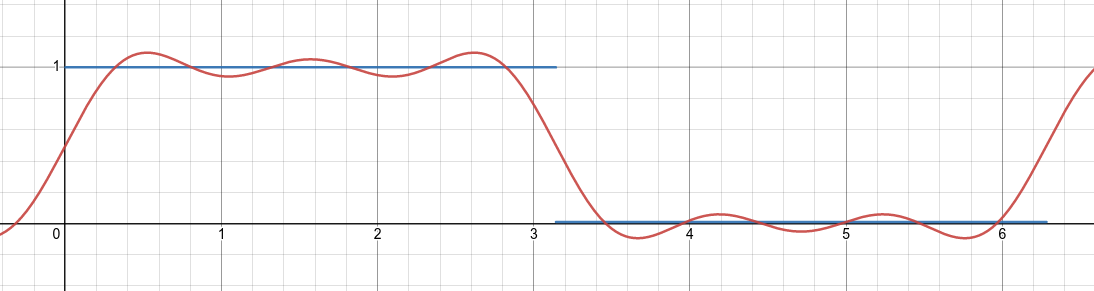
\includegraphics[width=.8\textwidth]{Dateien/Fourier_Beispiel.png}
\end{center}
Wie auf dem Bild zu sehen, approximieren wir mit jeden neuen Term die Funktion stückweise besser.

\end{Beispiel}
\begin{Satz}{Bemerkung}{Wichtige Fourier-Integrale}
Die folgenden Integrale sind sehr wichtig bei der Berechnung von Fourier-Reihen:
\begin{enumerate}
    \item $\int_0^{2\pi} \cos(kx)\sin(lx)dx=0, \mbox{ für $\forall k,l$}$
    \item $\int_0^{2\pi}\cos(kx)\cos(lx)dx=0 \mbox{ für $k\neq l$}$
    \item $\int_0^{2\pi}\sin(kx)\sin(lx)dx=0 \mbox{ für $k\neq l$}$
    \item $\int_0^{2\pi}\sin^2(kx)dx=\pi \mbox{ für $k\geq 1$}$
    \item $\int_0^{2\pi}\cos^2(kx)dx=\pi \mbox{ für $k\geq 1$}$
\end{enumerate}
\red{Wichtig!} Diese Beziehungen gelten nur für $k,l\in\N$.
\end{Satz}
\begin{Satz}{Bemerkung}{Fourier für un- und gerade Funktionen}
Es gilt $$F_n(f)=\frac{a_0}{2}+\sum_{k=1}^n (a_k\cos(kx)+b_k\sin(kx))$$
wobei $$a_k= c_k+c_{-k}=\frac{1}{\pi}\int_0^{2\pi}f(x)\cos(kx)dx$$
$$b_k=i(c_k-{c-k})=\frac{1}{\pi}\int_0^{2\pi}f(x)\sin(kx)dx$$
Wenn $f$ reellwertig ist, dann ist $c_{-k}=\overline{c_k}$ und $F_n(f)$ auch reellwertig. \\ \\
Ist $f$ gerade (d.h. $f(-x)=f(x)$), dann gilt
$$F_n(f)=\frac{a_0}{2}+\sum_{k=1}^n a_k\cos{(kx)}$$
Ist $f$ ungerade (d.h. $f(-x)=-f(x)$), dann gilt
$$F_n(f)=\sum_{k=1}^n b_k\sin{(kx)}$$
\end{Satz}
Eine weitere Anwendung der Fourier-Reihe ist auch das Beweisen von Folgen
\begin{Beispiel}{Folgenbeweise mit Fourier}
Wir sollen die Formel $\frac{\pi^2}{6}=1+\frac{1}{4}+\frac{1}{9}+\dots$ beweisen indem wir die Fourier-Reihe der $2\pi$-periodischen Funktion $f(x)=x^2$ im Intervall $-\pi\leq x\leq \pi$ bestimmen.
$$c_0=\frac{1}{2\pi}\int_{-\pi}^{\pi}x^2e^0dx=\frac{1}{2\pi}[\frac{x^3}{3}]_{-\pi}^{\pi}=\frac{1}{2\pi}(\frac{\pi^3}{3}+\frac{\pi^3}{3})=\frac{\pi^2}{3}$$
$$c_k=\frac{1}{2\pi}\int_{-\pi}^{\pi}x^2e^{-ikx}dx=\frac{1}{k^2}$$
$$c_k=\begin{cases} \frac{1}{k^2} & \mbox{wenn $k$ gerade} \\
-\frac{1}{k^2} & \mbox{wenn $k$ ungerade}
\end{cases}$$
$$F_n(f)=\frac{\pi^2}{3}-2\cos(x)+\frac{1}{2}\pi\cos(2x)-\frac{2}{9}\cos(3x)+\dots$$
Nun setzen wir für $x$ den Wert $x=\pi$ ein und erhalten:
$$F_n(f(\pi))=\frac{\pi^2}{3}+2+\frac{1}{2}+\frac{2}{9}+\dots$$
Wir wissen, dass $f(\pi)=\pi^2$ und substrahieren $\frac{\pi^2}{3}$ von beiden Seiten
$$\frac{\pi^2}{3}=2+\frac{1}{2}+\frac{2}{9}+\dots$$
Nun teilen wir beide Seiten mit $2$ und erhalten
$$\frac{\pi^2}{6}=1+\frac{1}{4}+\frac{1}{9}+\dots$$
\end{Beispiel}




\subsection{Konvergenz der Fourier Reihe}\label{ssec:FourierKonv}
\begin{Def}
{2-Norm}
Sei $V$ der Vektorraum der $2\pi$-periodischen Funktionen $f:\R \rightarrow \C$, wobei $f$ Riemann-integrierbar ist. Dann ist die Hermitische Form 
$$||f||_2=\langle f,f\rangle = \frac{1}{2\pi}\int_0^{2\pi}f(x)\overline{f(x)}dx, \space f\in V$$
die \red{2-Norm} von $f$.
\end{Def}
\begin{Satz}{Satz}{Konvergenz der Fourier-Reihe im quadratischen Mittel}
Sei $V$ der Vektorraum der $2\pi$-periodische Funktionen $f:\R\rightarrow\C$, für die $f$ integrierbar ist. \\
i) Für $\forall f\in V$ gilt
$$||f||_2^2=\sum_{k=-\infty}^\infty |c_k|^2$$
ii) Die Fourier-Reihe von $f\in V$ konvergiert im quadratischen Mittel gegen $f$, d.h. $\lim_{n\rightarrow \infty}||f-F_n(f)||_2=0$.
\end{Satz}
Es gibt tatsächlich keine $2\pi$-periodische Funktion im $\mathcal{L}^2$, dessen Fourier-Reihe nicht fast überall konvergieren würde.
%%%%%%% Damit fangen wir nächste Woche an %%%%%%%%
\newpage
\newpage
\section[Einführung in die Gebietsintegrale]{Mehrdimensionale Integrale}
\subsection{Theoretisches Baukasten}
Um uns mit mehrdimensionalen Integralen zu beschäftigen, müssen wir zuerst gewisse theoretische Begriffe einführen.
\begin{Def}{Charakteristische Funktion}
Sei $A\subseteq \R^n$. Die charakteristische Funktion \textit{oder auch} \red{Indikatorfunktion} der Teilmenge $A$ ist die Funktion
$$1_A:\R^n \rightarrow \R \mbox{ mit } x\rightarrow \begin{cases}1, x\in A \\
0, x\notin A\end{cases}$$
\end{Def}
\begin{Def}{Quader}
Ein \red{Quader} $Q\subseteq \R^n$ ist das Produkt $I_1\times \cdots \times I_n$ von $n$ beschränkten, nicht-leeren Intervallen $I_\mu \subseteq \R$.
\end{Def}
\begin{Beispiel}{Quader in $\R^1$}
Quader in $\R^1$ sind also die Intervale $(a,b)$, $[a,b]$, $(a,b]$ und $[a,b)$. \\
\end{Beispiel}
\begin{Def}{Volumen eines Quaders}
Das (n-dimensionale) Volumen eines solchen Quaders ist die nicht-negative reelle Zahl
$$v(Q)=v_n(Q)=\prod_{\mu = 1}^n |I_\mu|=\prod_{\mu = 1}^n (b_\mu - a_\mu)$$
\end{Def}
\begin{Def}{Treppenfunktion}
Eine Funktion $\varphi:\R^n \rightarrow \C$ heißt \red{Treppenfunktion auf $\R^n$}, wenn es endlich viele paarweise \textbf{disjunkte} Quader gibt, sodass
\begin{enumerate}[a)]
    \item die Funktion $\varphi$ auf jedem Quader $Q_k$ konstant ist,
    \item $\varphi(x)=0$ für alle $x$ außerhalb von Quadern.
    \end{enumerate}
Außerdem lassen sich Treppenfunktionen als endliche Linearkombination charakteristischer Funktionen von disjunkten Quadern schreiben
$$\varphi=\sum_{k}c_k 1_{Q_k} \mbox{ mit $c_k\in \C$ und $Q_k$ ist ein Quader}$$ 
\end{Def}
Wir kommen nun zu den sehr wichtigen Begriff der Hüllreihen.
\begin{Def}{Hüllreihe}
Gegeben sei $f:\R^n\rightarrow\C\cup \{\infty\}$. Eine \red{Hüllreihe} zu $f$ ist eine Reihe
$$\Phi=\sum_{k=1}^\infty c_k1_{Q_k} \mbox{ mit $c_k\in \R$}$$
wobei $Q_k$ \textbf{offene} Quader im $\R^n$ sind und für jedes $x\in\R^n$ gilt
$$|f(x)|\leq \Phi(x) = \sum_{k=1}^\infty c_k1_{Q_k}(x)$$
Der \red{Inhalt} der Hüllreihe ist definiert als
$$I(\Phi) = \sum_{k=1}^\infty c_k v(Q_k)$$
\end{Def}

\begin{Beispiel}{Folge von Hüllreihen}
Seien $a, k\in \R$ und $f:\R\rightarrow\R$ definiert als $f(x)=\begin{cases}0, x\neq a & k, x=a\end{cases}$. Wir sollen zu dieser Funktion eine Folge von Hüllreihen, $\Phi_n$, konstruieren, die gegen Null konvergiert. \\
Wir wissen, dass $\Phi = \sum_{k=1}^\infty c_k 1_{Q_k}$, aber auch, dass $c_k=0$ für jeden Quader außer für die, in denen sich $a$ befindet (da ist $c_k=k$). Wir können Hüllen als Intervale bilden und bekommen die Hüllreihe:
$$A_n=[a-\frac{1}{n}, a+\frac{1}{n}]$$
Die Inhalte dieser Hüllreihe gehen gegen 0
$$\lim_{n\rightarrow\infty}I(A_n)=\lim_{n\rightarrow\infty} a+\frac{1}{n}-(a-\frac{1}{n})=\lim_{n\rightarrow\infty}\frac{2}{n}=0$$
Wir haben nun erfolgreich eine Folge von Hüllreihen konstruiert
$$\Phi_n=\sum_{n=1}^\infty A_n$$
\red{muss noch verifiziert werden}
\end{Beispiel}
\begin{Beispiel}{Hüllreihe einer Funktion}
Wir betrachten die Funktion 
\begin{equation*}
  f(x)=\begin{cases}
    x & \mbox{wenn $x\in [0,1]$} \\
    0 & \mbox{sonst}
\end{cases}  
\end{equation*}
Dazu konstruieren wir eine Hüllreihe:
            \begin{center}
    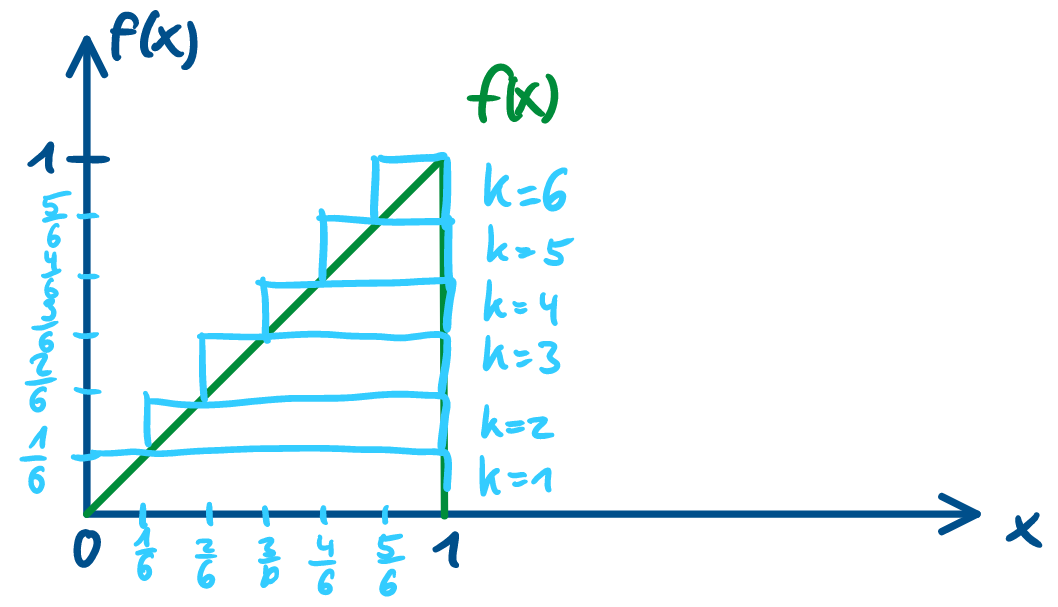
\includegraphics[width=0.80\textwidth]{Dateien/Hullreihe.png}
\end{center}
diese hat nun die Form $$\Phi_6(x)=\sum_{k=0}^{6-1}\frac{1}{6}\cdot 1_{[\frac{1}{6}k, 1]}$$ Lassen wir eine beliebige Anzahl $n$ an Quadern zu, gilt:
$$\Phi_n(x)=\sum_{k=0}^{n-1}\frac{1}{n}1_{[\frac{1}{n}k, 1]}$$
Der Inhalt ist dann
$$I(\Phi_n)=\frac{1}{n}\sum_{k=0}^{n-1} 1 -\frac{1}{n}k=\frac{1}{n}\sum_{k=0}^{n-1} 1 - \frac{1}{n^2}\sum_{k=0}^{n-1} k$$
$$=1-\frac{n-1}{2n}=\frac{1}{2}(1+\frac{1}{n})$$
Für $n\rightarrow \infty$ folgt:
$$I(\Phi_\infty)=\lim_{n\rightarrow\infty} \frac{1}{2}(1+\frac{1}{n})=\frac{1}{2}$$
Also dem Flächeninhalt unter der Funktion f!
\end{Beispiel}
\begin{Def}{$L^1$-Halbnorm}
Unter der \red{$L^1$-Halbnorm} von $f:\R^n\rightarrow\C\cup \{\infty\}$ versteht man das Infimum
$$||f||_1=\inf\{I(\Phi) |\mbox{ $\Phi$ Hüllreihe zu $f$} \}=\int |f|dx$$
\end{Def}
\begin{Satz}{Satz}{Eigenschaften einer Halbnorm}
Für die Funktionen $f_1, f_2: \R^n\rightarrow \C\cup\{\infty\}$ und ein $c\in\C$ gilt
\begin{enumerate}
\item $||c\cdot f||_1 = |c|\cdot ||f||_1$
\item $|f_1| \leq |f_2|  \implies ||f_1||_1 \leq ||f_2||_2$
\item $||\sum_{k=1}^\infty |f_k| ||_1\leq \sum_{k=1}^\infty ||f_k||_1$
\end{enumerate}
\end{Satz}
\newpage
\subsection{Lebesgue-Integral}
Mit den obigen theoretischen Werkzeug können wir nun endlich das Lebesgue-Integral definieren.
\begin{Def}{Lebesgue-Integral}
Eine Funktion $f:\R^n\rightarrow\C\cup\{\infty\}$ heißt \red{Lebesgue-integrierbar} über $\R^n$, wenn es eine Folge von Treppenfunktionen $\varphi_k$ gibt mit
$$\lim_{k\rightarrow \infty}||f-\varphi_k||_1=0$$
In diesem Fall schreiben wir das \red{Lebesgue-Integral}
$$\int fdx = \int f(x) d^nx = \int_{\R^n} f(x)dx = \lim_{k\rightarrow\infty} \varphi_k(x)dx\in\C$$
\end{Def}
\begin{Satz}{Satz}{Bedingte Gleichheit der Riemann und Lebesgue Integrale}
Sei $A=[a,b]$ ein kompaktes Intervall und $f$ eine über $A$ Riemann-integrierbare Funktion. Dann ist $f$ über $A$ Lebesgue-integrierbar und das Lebesgue-Integral und das Riemann-Integral sind gleich.
\end{Satz}
Der folgende zwei Sätze sind sehr wichtig in der Theorie der Gebietsintegrale. Im Skript stehen der kleiner und großer Satz von Fubini, wir schreiben hier aber die allgemeine Version aus T. Arens, also guckt euch auch das Skript nochmal an.
\begin{Satz}{Satz}{Kleiner Satz von Beppo Levi}
Sei $f:\R^n\rightarrow \R\cup \{\infty\}$ und sei $(\varphi_k)$ eine monoton wachsende oder fallende Folge von Treppenfunktionen, so dass
\begin{enumerate}[a)]
    \item $(\varphi_k)$ punktweise gegen $f$ konvergiert
    \item die Folge ($\int \varphi_k dx$) der Integrale der Treppenfunktionen beschränkt ist.
    Dann ist $f$ integrierbar und es gilt
    $$\int f dx=\lim_{k\rightarrow \infty}\int \varphi_k dx$$
\end{enumerate}
\end{Satz}
\begin{Satz}{Satz}{Satz von Fubini}
Sind $I\subseteq R^p$ und $J\subseteq R^q$ (möglicherweise unbeschränkte) Quader sowie $f\in L(Q)$ eine auf dem Quader $Q=I\times J \subseteq R^{p+q}$ integrierbare (oder mindestens stetig beschränkte) Funktion, so gibt es Funktionen $g\in L(I)$ und $h\in L(J)$ mit
$$g(x)=\int_J f(x,y) dy \mbox{ für fast alle $x\in I$}$$
$$h(y)=\int_I f(x,y)dx \mbox{ für fast alle $y\in J$}$$
Ferner ist 
$$\int_R f(x,y) d(x,y) = \int_I\int_J f(x,y) dy dx = \int_I g(x) dx$$
$$=\int_J\int_I f(x,y) dx dy = \int_J h(y) dy$$

\end{Satz}
\red{Wichtig!} Um den Satz von Fubini anwenden zu können, muss folgendes erwähnt werden:
\begin{itemize}
    \item $Q$ ist kompakt oder offen und beschränkt und
    \item $f$ ist stetig.
\end{itemize}
\begin{Beispiel}{Kompakte Kreissscheibe}
    Gegeben ist die kompakte Kreisscheibe:
    $$K=\overline{B_r(0)}=\{(x,y)\in\R^2| x^2+y^2\leq r^2\}$$
    Wir wollen nun das Integral
    $$\int_K 1 d(x,y)$$
    berechnen. Dazu stellen wir fest:
    \begin{enumerate}
        \item K ist kompakt
        \item $f(x,y)= 1$ ist stetig und beschränkt
        \item Die Menge $K_y$ lautet:
        $$K_y=\{x\in \R| (x,y)\in K\}=\{ x\in \R | x^2+y^2 \leq r^2\}$$
        $$= \{x\in \R | |x| \leq \sqrt{r^2-y^2}\}=[-\sqrt{r^2-y^2}, \sqrt{r^2-y^2}]$$
    \end{enumerate}
    Man erkennt leicht, dass $K_y\neq \emptyset$ für $y\in [-r, r]$. Somit erhalten wir:
    \begin{equation}
        F(y)=\begin{cases}\int_{K_y} 1dx & \mbox{ für $y\in [-1, 1]$} \\0 & \mbox{sonst}\end{cases}
    \end{equation}
    und damit nach dem Satz von Fubini:
    $$\int_K 1 d(x,y) = \int_\R F(y) dy = \int_{[-1,1]}[\int_{[-\sqrt{r^2-y^2}, \sqrt{r^2-y^2}]} 1dx]dy= \int_{-1}^{1} [\int_{-\sqrt{r^2-y^2}}^{\sqrt{r^2-y^2}} 1dx]dy=\pi r^2$$
    Eine nützliche Integrationsregel \red{$\int \sqrt{a^2-x^2}=\frac{1}{2}(a^2\sin^{-1}(\frac{x}{a})+x\sqrt{a^2-x^2})+c$}.
\end{Beispiel}
\begin{Beispiel}{Anwendung vom Satz von Fubini}
Wir wollen auch für eine kompliziertere Funktion, aber noch stets definiert auf einem Rechteck, die interierten Integrale berechnen. Dazu betrachten wir $R=(0,\frac{\pi}{2})\times (0,\frac{\pi}{2}$ und die Funktion $f:R\rightarrow \R$, die durch
$$f(x)=\sin(x_1+2x_2), \mbox{ $x=(x_1,x_2)\in R$}$$
gegeben ist. \\
Zunächst berechnen wir
$$\int_0^{\frac{\pi}{2}}\int_0^{\frac{\pi}{2}} \sin(x_1+2x_2)dx_2dx_1$$
$$=\int_0^{\frac{\pi}{2}}[-\frac{1}{2}\cos(x_1+2x_2)]^{\frac{\pi}{2}}_{x_2=0}dx_1$$
$$=\int_0^{\frac{\pi}{2}}(\frac{1}{2}\cos(x_1)-\frac{1}{2}\cos(x_1+\pi))dx_1$$
$$=\int_0^{\frac{\pi}{2}}\cos(x_1)dx_1 = 1$$
Nun vertauschen wir die Reihenfolge,
$$\int_0^{\frac{\pi}{2}}\int_0^{\frac{\pi}{2}} \sin(x_1+2x_2)dx_1dx_2$$
$$=\int_0^{\frac{\pi}{2}} [-\cos(x_1+2x_2)]^{\frac{\pi}{2}}_{x_1=0}dx_2$$
$$=\int_0^{\frac{\pi}{2}} (\cos(2x_2)-\cos(2x_2+\frac{\pi}{2}))dx_2$$
$$=[\frac{1}{2}\sin(2x_2)-\frac{1}{2}\sin(2x_2+\frac{\pi}{2})]_0^{\frac{\pi}{2}}$$
$$=\frac{1}{2}(\sin(\pi)-\sin(\frac{3\pi}{2})-\sin(0)+\sin(\frac{\pi}{2})) = 1$$
\end{Beispiel}
\begin{Beispiel}{Fubini ist nicht immer anwendbar}
\begin{center}
    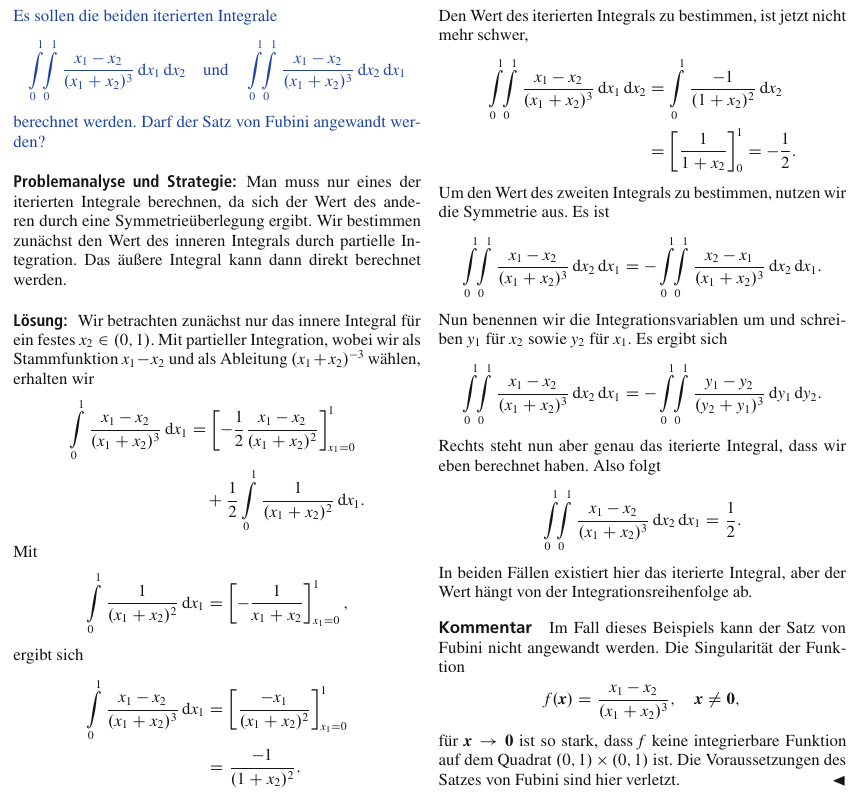
\includegraphics[width=\textwidth]{Dateien/Fubini2.png}
\end{center}
\end{Beispiel}
\newpage
\subsection{Volumina und Nullmengen}

Wir beginnen dieses wichtige Thema mit sehr theoretischen Konzepten, die uns dann ermöglichen die Maßtheorie zu verstehen. So manche Begriffe werden in der Funktionalanalysis in MfP4 nochmal vorkommen.
\begin{Def}{Grundmenge und $\sigma$-Algebra}
Eine \red{Grundmenge} (auch Universum), $\Omega$, bezeichnet in der Mathematik eine Menge aus allen in einem bestimmten Zusammenhang betrachteten Objekten. \\
Eine Menge $\mathcal{A}$ von Teilmengen einer Grundmenge $\Omega$ heißt \red{$\sigma$-Algebra}, wenn
\begin{itemize}
    \item $\Omega \in \mathcal{A}$
    \item Für jede Menge $A\in \mathcal{A}$ gilt $\Omega / A\in \mathcal{A}$
    \item Abzählbare Vereinigungen von Mengen $A_i\in \mathcal{A}$ sind wieder in $\mathcal{A}$
\end{itemize}
\end{Def}
\begin{Beispiel}{Kleinste und größte $\sigma$-Algebra}
Für jede beliebige Menge $\Omega$ ist $\{\emptyset, \Omega\}$ die kleinste und die Potenzmenge $P(\Omega)$ die größtmögliche $\sigma$-Algebra mit $\Omega$ als Grundmenge.
\end{Beispiel}
\begin{Def}{Maß}
Sei $\mathcal{A}$ eine $\sigma$-Algebra. Eine Funktion $\mu: \mathcal{A}\rightarrow[0,\infty]$ heißŧ ein \red{Maß} auf $\mathcal{A}$, wenn
\begin{itemize}
    \item $\mu(\emptyset)=0$,
    \item $\sigma$-Additivität, also $\mu(\cup_{n=1}^\infty A_n)=\sum_{n=1}^\infty \mu(A_n)$.
\end{itemize}
Außerdem wird das Tripel $(\Omega, \mathcal{A}, \mu)$ \red{Maßraum} gennant.
\end{Def}
\begin{Beispiel}{Borelsche $\sigma$-Algebra}
Die \red{borelsche $\sigma$-Algebra} ist eine $\sigma$-Algebra, die alle Mengen enthält, denen man naiverweise ein Volumen oder eine Wahrscheinlichkeit zuordnen will, schließt aber Negativresultate aus. \\
Bezüglich der borelschen $\sigma$-Algebra sind alle stetigen Funktionen immer messbar.
\end{Beispiel}
\begin{Def}{$\sigma$-Kompaktheit}
    Eine Menge $A\subseteq \R^n$ heißt \red{$\sigma$-kompakt}, wenn sie eine Vereinigung abzählbar vieler kompakter Menger ist.
\end{Def}
Nun kommt eine sehr wichtige Definition.
\begin{Def}{Lebesgue-Messbarkeit}
Eine Menge $A\subseteq \R^n$, falls die konstante Funktion über $A$ integrierbar ist.
$$v(A)=v_n(A)=\int_A 1dx$$
\end{Def}
\begin{Def}{Figur und Ausschöpfung}
Eine Vereinigung endlich vieler Quader $Q_i\subseteq \R^n$ der Form $A=Q_1\cup Q_2 \cup \dots \cup Q_s$ heißt \red{Figur}. \\
Eine \red{Ausschöpfung} von $A$ ist eine aufsteigende Folge von Teilmengen $A_1\subseteq A_2 \subseteq \cdots \subseteq A$.
\end{Def}
\begin{Beispiel}{Volumen von Kegeln}
WIP
\end{Beispiel}
Und nun eins der wichtigsten Definitionen im MfP3.
\begin{Def}{Nullmenge}
Eine Teilmenge $N\subseteq \R^n$ heißt Lebesgue-Nullmenge, wenn sie eine der beiden folgenden Bedingungen erfüllt:
\begin{itemize}
    \item $N$ ist messbar mit $v_n(N)=0$.
    \item Für die charakteristische Funktion gilt $||1_{N}||_1=0$.
\end{itemize}
\end{Def}
\begin{Beispiel}{Nullmengen}
Überlegen Sie sich einige Beispiele für Nullmengen im $\R^2$ und im $\R^3$. \\ \\
In jedem Fall sind isolierte Punkte und abzählbare Vereinigungen von isolierten Punkten wie im eindimensionalen Nullmengen. Das bedeutet etwa, dass $\Q^2\subset \R^2$ oder $\Q^3 \subset \R^3$ Nullmengen sind. \\ \\
Der Rand eines Quaders, im zweidimensionalen also der Rand eines Rechtecks, ist ebenfalls eine Nullmenge. Dasselbe gilt für abzählbare Vereinigungen solcher Ränder. \\ \\
Als letztes Beispiel im $\R^2$ sei der Graph einer Funktion $f:\R\rightarrow \R$ gennant.
\end{Beispiel}
\begin{Def}{Fast überall}
Sei $E(x)$ eine Eigenschaft, sodass wir für $\forall x \in \R^n$ wissen, ob die Eigenschaft $E(x)$ erfüllt ist. Wir sagen, dass $E(x)$ \red{fast überall} gilt, wenn die Menge aller Punkte, wo $E(x)$ nicht gilt, eine Nullmenge ist.
\end{Def}
\begin{Beispiel}{Fast überall konstante Funktion}
Sei $f(x)=\begin{cases}42 \mbox{ wenn $x\neq \infty$} \\
\infty \mbox{ wenn $x=\infty$}\end{cases}$. Die Funktion $f(x)$ ist fast überall konstant, außer in einer Nullmenge (also in der Unendlichkeit). 
\end{Beispiel}
Es ist auch nützlich sich zu merken, dass wenn $||f||_1=0$, dann $N=\{ x\in \R^n | f(x)\neq 0\}$ eine nullmenge ist.
\begin{Satz}{Satz}{Modifikationssatz}
Seien $f,g:\R^n\rightarrow \C$ zwei Funktionen, die fast überall gleich sind. Wenn $f$ integrierbar ist, dann ist auch $g$ integrierbar und es gilt $\int f = \int g$.
\end{Satz}
\begin{Satz}{Lemma}{Geometrische Charakterisierung von Nullmengen}
    Ist $N$ eine Nullmenge, so gibt es zu jedem $\epsilon>0$ eine messbare offene Menge $U$ mit $N\subseteq U$ und $v(U)<\epsilon$. \\
    Eine Menge $N\subseteq \R^n$ ist genau dann eine Nullmenge, wenn es zu jedem $\epsilon>0$ abzählbar viele Quader $Q_1, Q_2, ..., Q_n$ gibt, sodass
    $$N\subseteq \bigcup_{k=1}^{\infty}Q_k \mbox{ und }\sum_{k=1}^\infty v(Q_k)>\epsilon$$
\end{Satz}
Eine nützliche, aber nicht so wichtige Eigenschaft ist, dass wenn $f$ integrierbar ist, dann auch $f(x-a)$ integrierbar ist, wenn $a$ in der Definitionsmenge ist.
\newpage
\subsection{Konvergenzsätze}
Zuerst wollen wir uns an die punktweise und gleichmäßige Kovergenz aus MfP2 erinnern.
\begin{Def}
{Gleichmäßige Konvergenz}
Sind $(X,d_X)$ und $(Y,d_Y)$ metrische Räume und $(f_n:X\to Y)_{n\in\mathbb{N}}$ eine Folge von Abbildungen.\\
Wir sagen, dass $f$ genau dann \red{gleichmäßig} gegen eine Grenzfunktion $f$ \red{konvergiert}, wenn es für alle $\epsilon>0$ ein $N=N(\epsilon)\in\mathbb{N}$ gibt, sodass
\begin{equation*}
    d_Y(f_n(x),f(x))<\epsilon\quad \forall n\geq N\land \forall x\in X.
\end{equation*}
\end{Def}
\begin{Def}
{Punktweise Konvergenz}
Eine Folge $(f_n)$ von Abbildungen \red{konvergiert punktweise} gegen eine Abbildung $f$, falls $\lim_{n\to\infty}f_n(x)=f(x)\,\forall x\in X$.
\end{Def}
\begin{Beispiel}
    {Gleichmäßige Konvergenz}
    Wir betrachten die Funktionenfolge
    \begin{equation*}
        f_n(x)=\sqrt{\vert x \vert^2 + \frac{1}{n^2}} \qquad x \in \mathbb{R}.
    \end{equation*}
    Konvergiert diese Folge gleichmäßig gegen eine Grenzfunktion, sagen wir $f(x)=\vert x \vert$? In weiser Voraussicht und um die weitere Rechnung plausibel zu machen, schauen wir uns zunächst die folgende Ungleichung an: 
    \begin{equation*}
        \sqrt{a+b} \leq \sqrt{a+b+2\sqrt{ab}} = \sqrt{(\sqrt{a}+\sqrt{b})^2}=\sqrt{a}+\sqrt{b}.
    \end{equation*} \\
    
    Damit können wir nun recht schnell nachprüfen:
    \begin{align*}
        \forall \epsilon > 0 \,\exists N\in\mathbb{N}\, &\forall x\in D_f \,\forall n\geq N: \\
            &\vert f_n(x)-f(x) \vert = \bigl| \sqrt{\vert x \vert^2 + \frac{1}{n^2}} - \vert x \vert \bigr| \leq \bigl| \vert x \vert + \frac{1}{n} - \vert x \vert \bigr| = \frac{1}{n} \leq \frac{1}{N} < \epsilon
    \end{align*}
    Das Kriterium ist also erfüllt und die Funktion damit gleichmäßig konvergent (und daher auch automatisch punktweise konvergent), da wir die $x$-Abhängigkeit in der Abschätzung losgeworden sind.
\end{Beispiel}
Ebenso ein Beispiel, um uns auf die Quotientenvektorräume aus MfP2 zu erinnern.
\begin{Beispiel}{Quotientenvektorraum}
    Sei $V=\R^4$ und $U=span\{(1,1,0,0)^T, (0,1,-1,0)^T\}\subseteq V$ ein Untervektorraum. Wir sollen zeigen, dass im Quotientenvektorraum $U/V$ gilt
    $$[\begin{pmatrix}
        1 \\
        0 \\
        1 \\
        2 \\
    \end{pmatrix}]=[\begin{pmatrix}
        3 \\
        1 \\
        2 \\
        2 \\
    \end{pmatrix}] \mbox{ und }[\begin{pmatrix}
        1 \\
        0 \\
        1 \\
        0 \\
    \end{pmatrix}]\neq[\begin{pmatrix}
        1 \\
        0 \\
        0 \\
        0 \\
    \end{pmatrix}]$$
    Dabei bezeichnet [$v$] die Äquvialenzklasse von $v\inV$ von $V/U$. \\
    Ein Quotientenvektorraum besteht aus allen Vektoren $a,b\in V$ für die gilt $a+b\in U$.
    $$\begin{pmatrix}
        1 \\
        0 \\
        1 \\
        2 \\
    \end{pmatrix}+\begin{pmatrix}
        3 \\
        1 \\
        2 \\
        2 \\
    \end{pmatrix}=\begin{pmatrix}
        4 \\
        1 \\
        3 \\
        0 \\
    \end{pmatrix}$$
    Wir können nun den Vektor $\begin{pmatrix}
        4 \\
        1 \\
        3 \\
        0 \\
    \end{pmatrix}$ mit den Basisvektoren von $U$ darstellen
    $$\begin{pmatrix}
        4 \\
        1 \\
        3 \\
        0 \\
    \end{pmatrix}= a \begin{pmatrix}
        1 \\
        1 \\
        0 \\
        0 \\
    \end{pmatrix}+b\begin{pmatrix}
        0 \\
        1 \\
        -1 \\
        0 \\
    \end{pmatrix}$$
    Wenn wir $a=4$ und $b=1$ setzen, dann wird das Ungleichungssystem gelöst. Also stimmt die erste Äquivalenzklasse. Nun gucken wir uns das für die anderen zwei Vektoren an
    $$\begin{pmatrix}
        1 \\
        0 \\
        1 \\
        0 \\
    \end{pmatrix}+\begin{pmatrix}
        1 \\
        0 \\
        0 \\
        0 \\
    \end{pmatrix}=\begin{pmatrix}
        2 \\
        0 \\
        1 \\
        0 \\
    \end{pmatrix} \mbox{,     } \begin{pmatrix}
        2 \\
        0 \\
        1 \\
        0 \\
    \end{pmatrix}=a \begin{pmatrix}
        1 \\
        1 \\
        0 \\
        0 \\
    \end{pmatrix}+b\begin{pmatrix}
        0 \\
        1 \\
        -1 \\
        0 \\
    \end{pmatrix}$$
    Und wir merken schon, dass es keine $a$ und $b$ gibt, sodass das Gleichungssystem gelöst werden kann, daher gehören die letzten zwei Vektoren nicht zu der Äquvivalenzklasse.
\end{Beispiel}
Nun kommen wir zu sehr wichtigen Sätzen.
\begin{Satz}{Theorem}{Satz von Riesz-Fischer}
    Vorausgesetzt $f_k$ ist eine $\mathcal{L}^1$-Cauchy-Folge integrierbarer Funktionen, dann \begin{itemize}
        \item existiert $f\in \mathcal{L}^1(\R^n)$ mit $\lim_{k\rightarrow \infty}f_k = f$ mit $\int f dx = \lim_{k\rightarrow \infty}\int f_k dx$ und
        \item $(f_k)$ konvergiert punktweise gegen $f$.
    \end{itemize}
    Somit ist $\mathcal{L}^1(\R^n)$ ein Banachraum. Die \red{Vertauschbarkeit} von Integral und Limes folgt grob aus der Konvergenz bzgl. der $\mathcal{L}^1$-Halbnorm.
\end{Satz}
Beachtet, dass der $\mathcal{L}^1$- Grenzwert nicht eindeutig ist, aber es kann sein, dass sich die Grenzwerte nur auf eine Nullmenge unterscheiden.
\begin{Satz}{Satz}{Satz von Beppo-Levi von der monotonen Konvergenz}
    Voraussetzungen:
    \begin{itemize}
        \item $f_k:\R^n\rightarrow \R \cup \{ \infty\}$ ist monoton wachsende/fallende Folge integrierbarer Funktionen
        \item $f_k$ konvergiere punktweise gegen $f(x)=\lim_{k\rightarrow \infty} f_k(x)$
        \item Die Folge $\int f_k dx$ der Integrale ist beschränkt.
    \end{itemize}
    Dann folgt, dass $f$ integrierbar ist und dass $\int f dx = \lim_{k\rightarrow \infty} \int f_k dx$
\end{Satz}
\begin{Satz}{Satz}{Satz von Lebesgue von der majorisitierten Konvergenz}
    Voraussetzungen:
    \begin{itemize}
        \item $f_k:\R^n\rightarrow \C \cup \{ \infty\}$ ist eine Folge integrierbaren Funktionen
        \item $f_k$ konvergiert fast überall punktweise gegen eine Funktion $f$
        \item Es gibt eine integrierbare Majorante $F$ mit $|f_k|\leq F$ für $\forall k$.
    \end{itemize}
    Dann folgt, dass $f$ integrierbar ist und dass $\int f dx = \lim_{k\rightarrow \infty} \int f_k dx$
\end{Satz}
\begin{Beispiel}{Satz von integrierbaren Majoranten angewandt}
    Wir betrachten die Funktion
    $$\delta_n(x)=\begin{cases}
        xn^2 & 0\leq x< \frac{1}{n} \\
        2n-xn^2 & \frac{1}{n} \leq x \leq \frac{2}{n} \\
        0 & \mbox{sonst}
    \end{cases}$$
    Die Funktionenfolge ist unbeschränkt wie wir gesehen haben, da
    $$\max_{x\in\R} \delta_n(x)=n$$
    Es gibt also keine integrierbare Majorante und somit ist nicht sichergestellt, dass Integral und Limes vertauschen zu können. Tatsächlich gilt:
    $$\lim_{n\rightarrow \infty} \int_\R \delta_n(x) dx = 1 \mbox{ und } \int_\R \delta(x)dx = 0$$
\end{Beispiel}
\begin{Beispiel}{Und noch ein Beispiel}
    \begin{center}
    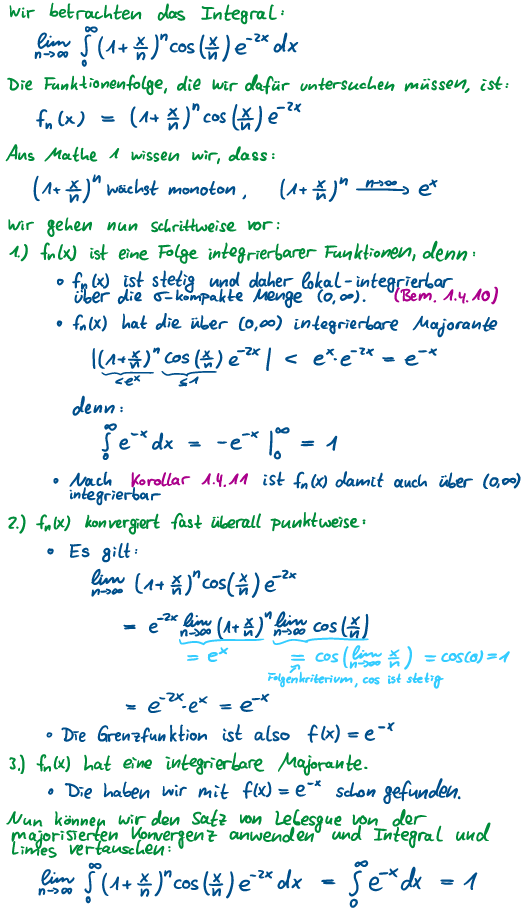
\includegraphics[width=0.80\textwidth]{Dateien/Beppo_Levi_Beispiel.png}
\end{center}
\end{Beispiel}
\newpage
\subsection{Parameterabhängige Integrale}
Die Vertauschbarkeit von Integral und Limes führt zu weiteren, sehr praktischen Sätzen.
\begin{Satz}{Satz}{Verallgemeineter Hauptsatz der Differential- und Integralrechnung}
Voraussetzungen:
\begin{itemize}
    \item $f$ ist differenzierbar auf dem kompakten Intervall $[x_0, x]$.
    \item Die Ableitung von $f$ ist beschränkt.
\end{itemize}
Daraus folgt, dass $f'$ Lebesgue-integrierbar ist über $[x_0, x]$ und dass $$f(x)-f(x_0)=\int_{[x_0, x]} f'(t)dt$$.
\end{Satz}
\begin{Satz}{Satz}{Stetigkeitssatz}
    Voraussetzungen:
    \begin{itemize}
        \item Sei $X$ ein metrischer Raum und $T\subseteq \R^p$
        \item $f:X\times T\rightarrow \C, (x,t)\longmapsto f(x,t)$ ist für feste $x$ über $T$ integrierbar
        \item Für feste $t$ ist die Funktion $x\longmapsto f(x,t)$ stetig
        \item Es gibt eine integrierbare Majorante $\Phi: T\rightarrow \R$, sodass $|f(x,t)|\leq \Phi(t)$ für $\forall (x,t)\in X\times T$.
    \end{itemize}
    Daraus folgt, dass $F(x)=\int_T f(x,t)dt$ ist auf $X$ stetig.
\end{Satz}
\begin{Satz}{Satz}{Differentiationssatz}
        Voraussetzungen:
    \begin{itemize}
        \item Sei $X\subseteq \R^n$ und $T\subseteq \R^p$
        \item $f: X\times T\rightarrow \C$, $(x,t)\rightarrow f(x,t)$ ist für feste $x$ über $T$ integrierbar
        \item Für feste $t$ ist die Funktion $x\longmapsto f(x,t)$ stetig diff'bar
        \item Es gibt eine intergierbare Majorante $\Phi:T\rightarrow \R$ mit
        $$|\frac{\partial f}{\partial v_\mu}(x,t)|\leq \Phi(t)\mbox{ für }\forall (x,t)\in X\times T\mbox{ für }\mu = 1,...,n$$
    \end{itemize}
    Daraus folgt, dass
    \begin{itemize}
        \item $F(x)=\int_T f(x,t)dt$ ist stetig diff'bar,
        \item $t\mapsto\frac{\partial}{\partial x_p}f(x,t)$ ist für jedes $x$ integrierbar und
        \item es gilt $\frac{\partial}{\partial x_\mu}\int_T f(x,t)dt=\int_T \frac{\partial}{\partial x_\mu} (x,t) dt$.
    \end{itemize}
\end{Satz}
\begin{Beispiel}{Fourier-Transformation}
        \begin{center}
    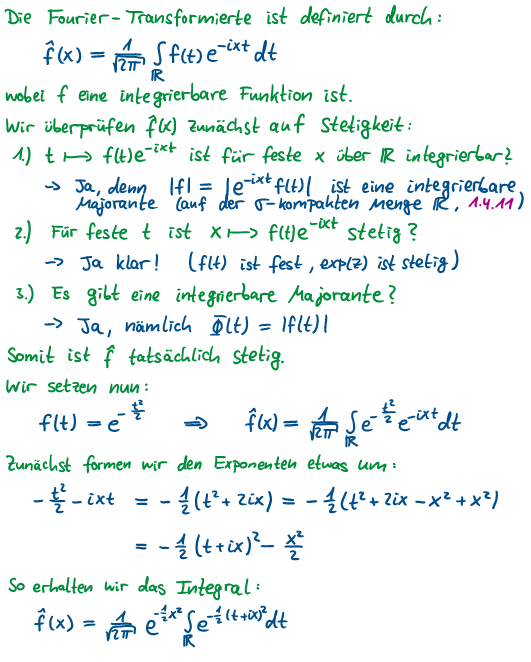
\includegraphics[width=0.80\textwidth]{Dateien/Fourier_Transform_1.png}
    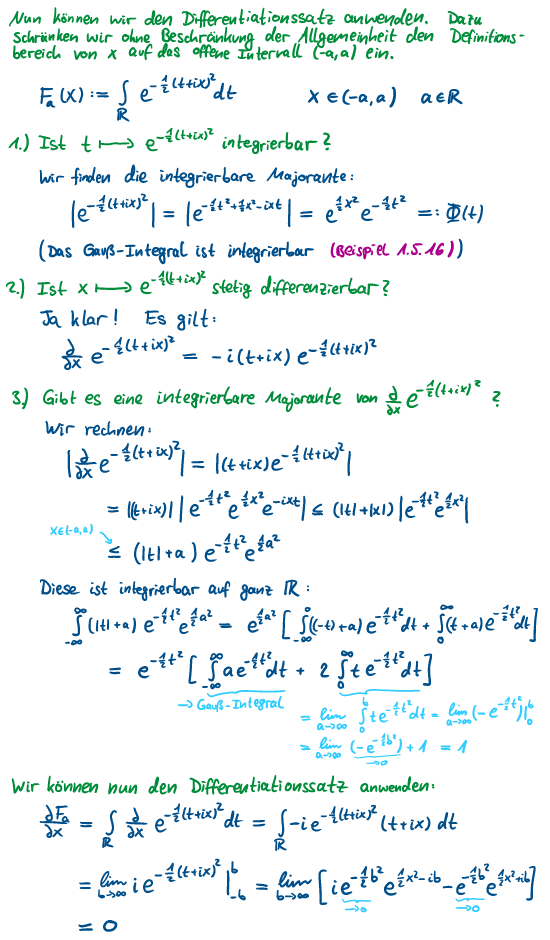
\includegraphics[width=0.80\textwidth]{Dateien/Fourier_Transform_2.png}
    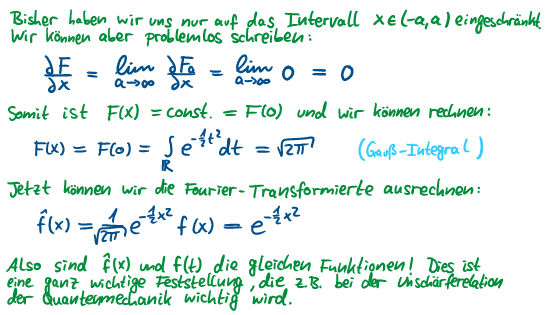
\includegraphics[width=0.80\textwidth]{Dateien/Fourier_Transform_3.png}
\end{center}
\end{Beispiel}
\newpage
Aus all diesen Sätzen kommt nun der Höhepunkt der Integrationstheorie. Die folgenden zwei Sätze sind von enormer bedeutung in der Physik, also merkt sie euch. 
\begin{Satz}{Satz}{Satz von Tonelli}
    Vorausgesetzt $f:\R^p\times \R^q \rightarrow \C$ ist fast überall stetig oder lokal integrierbar. Dann gilt die folgende Äquivalenz
    $$\int_{\R^q}(\int_{\R^p} |f(x,y)|dx)dy \quad\mbox{oder}\quad\int_{\R^p}(\int_{\R^q} |f(x,y)|dx)dy\mbox{ existiert} $$
    $$\iff \mbox{$f$ ist über $\R^p\times\R^q$ integrierbar}$$
\end{Satz}
\begin{Satz}{Satz}{Transformationssatz}
    Voraussetzung:
    \begin{itemize}
        \item $U,V\subseteq \R^n$ offen
        \item $T: U\rightarrow V$ ist ein Diffeomorphismus
        \end{itemize}
        Daraus folgen
    \begin{itemize}
            \item die Äquivalenz $f:V\rightarrow \C\cup\{\infty\}$ integrierbar $\iff f\circ T\cdot |\det(dT)|$ integrierbar
            \item $\int_u f(T(x))|\det(dT)|dx=\int_V f(y)dy$
        \end{itemize}
    
\end{Satz}
Zur Erinnerung die definition der allgemeinen linearen Gruppe: $$GL(n,\R)=\{A\in \mbox{Mat}(n,\R)| \det(A)\neq0\}$$
Außerdem nicht vergessen, dass der Betrag der Determinante einer Matrix das gerichtete Volumen eines Parallelepipeds darstellt.
\begin{Def}{Affine Transformationen}
    Voraussetzung:
    \begin{itemize}
        \item $T:\R^n\rightarrow \R^n$, $T(x)=Ax+b$ mit $A\in GL(n,\R), b\in \R^n$
        \item $f:K\rightarrow \C$ ist über $K\subseteq \R^n$ integrierbar
    \end{itemize}
    Daraus folgen
    \begin{itemize}
        \item $dT=A \Rightarrow \det(dT)=\det(A)\in \R/\{0\}$
        \item $f\circ T$ ist über $T^{-1}(K)$ integrierbar
        \item Es gilt $\int_{T^{-1}(K)} f(T(x)) dx = \frac{1}{|\det(A)|}\int_K f(y) dy$.
    \end{itemize}
\end{Def}
\begin{Beispiel}{Präsenzaufgabe 1 aus dem Blatt 6}
    \red{WIP}
\end{Beispiel}
\begin{Beispiel}{Bestimmung eines uneigentlichen Integrals}
    \begin{center}
    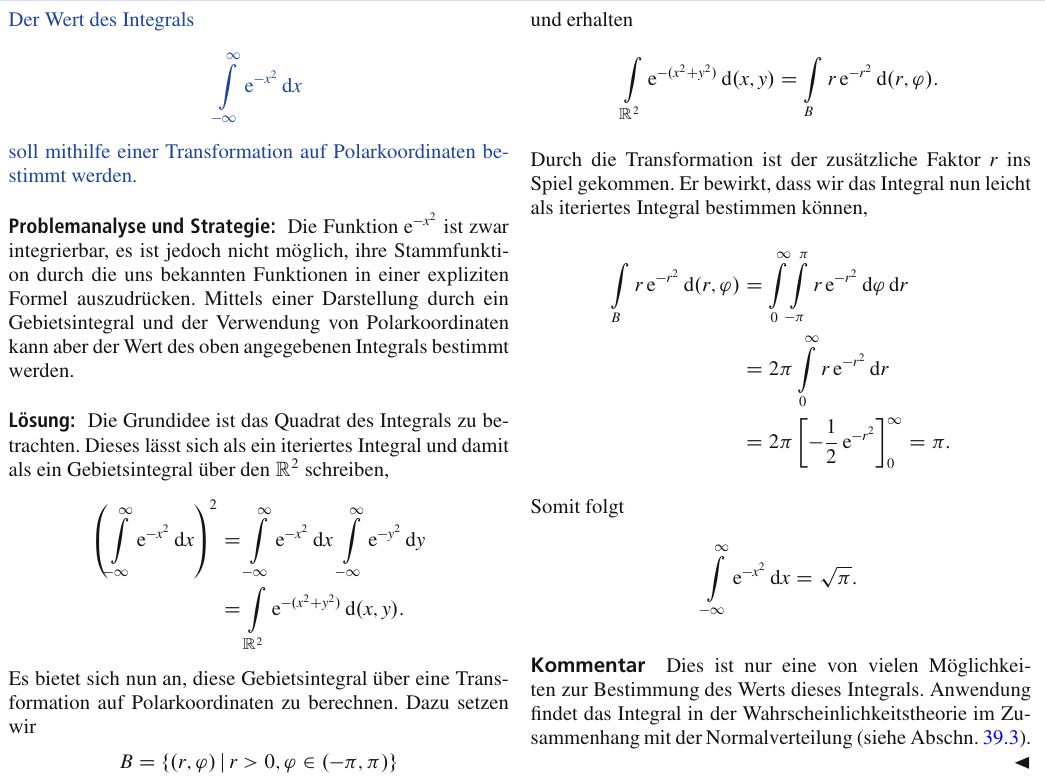
\includegraphics[width=0.95\textwidth]{Dateien/Uneigentlich_e_hoch_x_quadrat.png}

\end{center}
\end{Beispiel}
\begin{Beispiel}{Transformationssatz im Einsatz}
            \begin{center}
    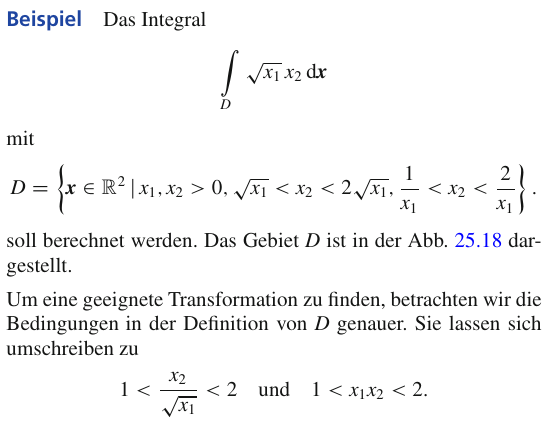
\includegraphics[width=0.52\textwidth]{Dateien/Transformationssatz1.png}
    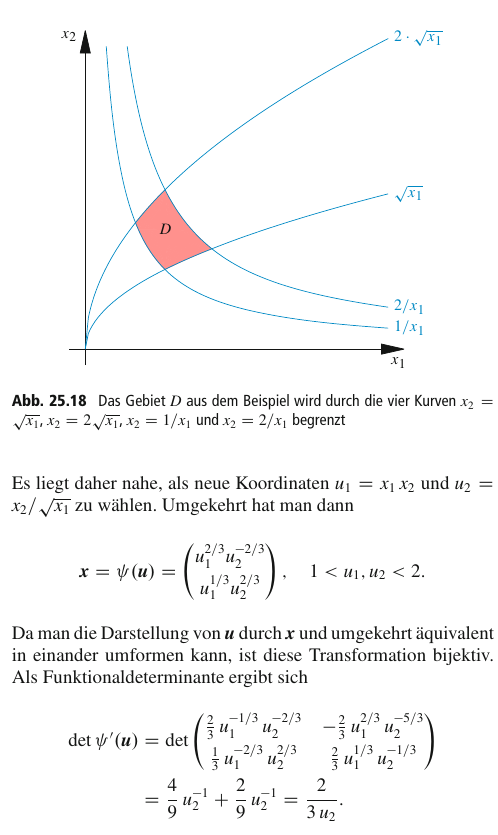
\includegraphics[width=0.52\textwidth]{Dateien/Transformationssatz2.png}
    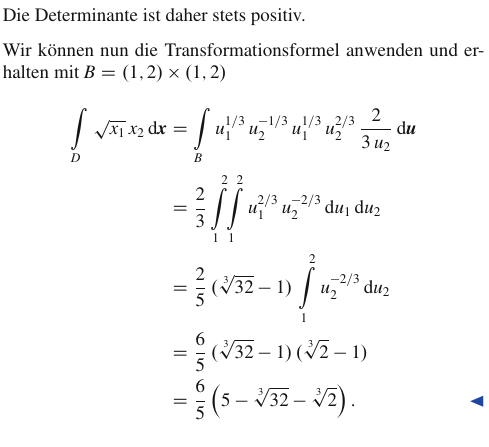
\includegraphics[width=0.52\textwidth]{Dateien/Transformationssatz3.png}
\end{center}
\end{Beispiel}
\newpage
\subsection{Exkurs: Wichtige Koordinatensysteme}
Dieses Thema ist euch allen schon aus der Physik 2 bekannt und könnt es überspringen, aber guck euch die Beispiele zur Erinnerung vor der Klausur nochmal an. \\
Für das \red{Polarkoordinatensystem} gelten die folgenden Gleichungen:
$$x_1=r\cos(\varphi)$$
$$x_2=r\sin(\varphi)$$
$$\Phi(r, \varphi) = \begin{pmatrix}
    r\cos(\varphi) \\
    r\sin(\varphi)
\end{pmatrix}$$
\begin{Def}{Integration mit Polarkoordinaten}
Ist $D\subseteq \R^2, f\in L(D)$ und $B$ die Beschreibung von $D$ durch Polarkoordinaten, so gilt
$$\int_D f(x_1,x_2)d(x_1,x_2) = \int_B f(r\cos(\varphi), r\sin(\varphi))rd(r, \varphi)$$
\end{Def}
\begin{Beispiel}{Integration mit Polarkoordinaten}
\begin{center}
    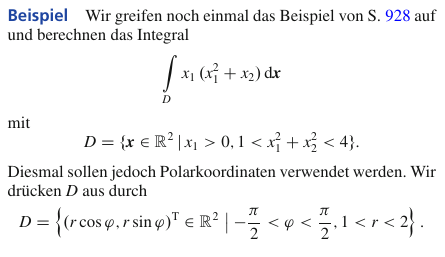
\includegraphics[width=0.52\textwidth]{Dateien/Polarkoord1.png}
    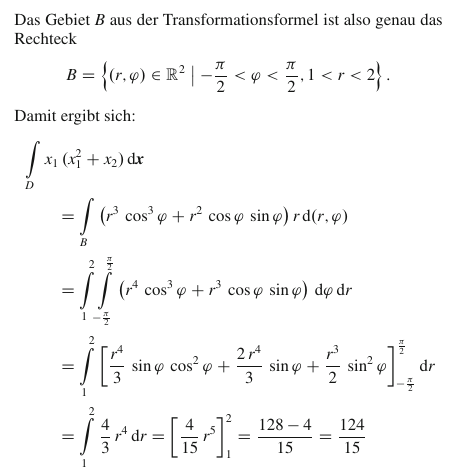
\includegraphics[width=0.52\textwidth]{Dateien/Polarkoord2.png}
\end{center}
\end{Beispiel}

Für das \red{Zylinderkoordinatensystem} gelten die folgenden Gleichungen:
$$x_1=\rho\cos(\varphi)$$
$$x_2=\rho \sin(\varphi)$$
$$x_3=z$$
$$\Phi(\rho, \varphi, z)=\begin{pmatrix}
    \rho \cos(\varphi) \\
    \rho \sin(\varphi) \\
    z
\end{pmatrix}$$
\begin{Def}{Integration mit Zylinderkoordinaten}
Ist $D\subseteq \R^3, f\in L(D)$ und $B$ die Beschreibung von $D$ durch Polarkoordinaten, so gilt
$$\int_D f(x_1,x_2,x_3)d(x_1,x_2,x_3) = \int_B f(\rho\cos(\varphi), \rho\sin(\varphi),z)\rho d(\rho, \varphi, z)$$
\end{Def}
\begin{Beispiel}{Integration mit Zylinderkoordinaten}
    \begin{center}
    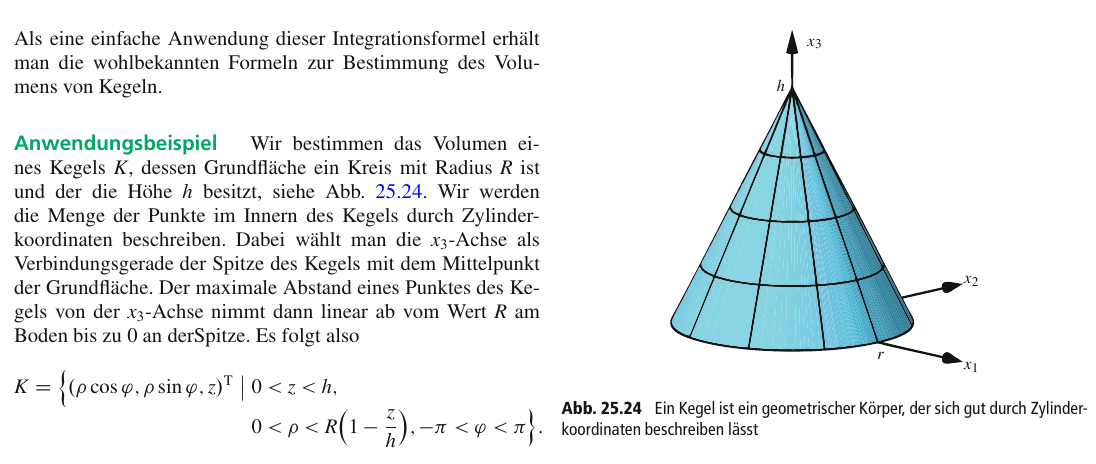
\includegraphics[width=1.0\textwidth]{Dateien/Zylinderkoord1.png}
    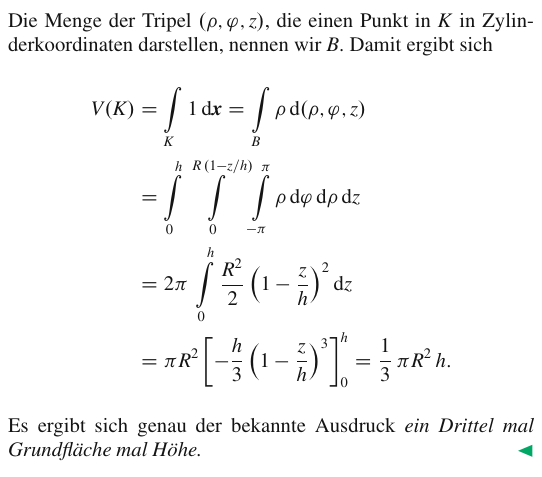
\includegraphics[width=0.7\textwidth]{Dateien/Zylinderkoord2.png}
\end{center}
\end{Beispiel}
Zum guten Letzt gelten für das \red{Kugelkoordinatensystem} die folgenden Gleichungen:
$$x_1=r\cos(\varphi)\sin(\theta)$$
$$x_2=r \sin(\varphi)\sin(\theta)$$
$$x_3=z\cos(\theta)$$
$$\Phi(r, \varphi, \theta)=\begin{pmatrix}
    r \cos(\varphi)\sin(\theta) \\
    r \sin(\varphi)\sin(\theta) \\
    r \cos(\theta)
\end{pmatrix}$$
\begin{Def}{Integration mit Kugelkoordinaten}
Ist $D\subseteq \R^3, f\in L(D)$ und $B$ die Beschreibung von $D$ durch Polarkoordinaten, so gilt
$$\int_D f(x_1,x_2,x_3)d(x_1,x_2,x_3) = \int_B f(r \cos(\varphi)\sin(\theta), r \sin(\varphi)\sin(\theta),r \cos(\theta))r^2\sin(\theta) d(r, \varphi, \theta)$$
\end{Def}
\begin{Beispiel}{Integration mit Kugelkoordinaten}
        \begin{center}
    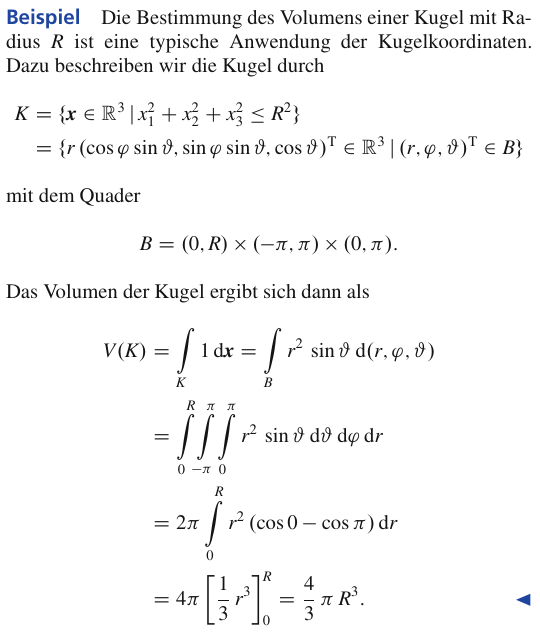
\includegraphics[width=0.7\textwidth]{Dateien/Kugelkoord.png}
\end{center}
\end{Beispiel}
\newpage
\section[Einführung in die Tensorprodukte]{Tensorprodukt}
\textit{Das Tensorprodukt verknüpft auf charakteristische Weise zwei Vektorräume miteinander. Die Definitionen mögen sehr trocken wirken, also wäre meine Empfehlung sich zuerst die Beispiele anzugucken und dann die Theorie anzupacken.}
\subsection{Mathematisches Tensorprodukt}
\begin{Def}{Tensorprodukt}
    Zunächst erweitern wir den Begriff der Billinearform. Statt
    $$\alpha: V\times W \rightarrow \mathbb{K}$$
    gilt nun:
    $$\alpha: V\times W \rightarrow X$$
    wobei $X$ ein Vektorraum ist. \\ \\
    Das \red{Tensorprodukt} kann man sich einfach als eine neue Verknüpfung zwischen Vektorräumen vorstellen. Sie ist definiert über die universelle Eigenschaft:
    \begin{center}
    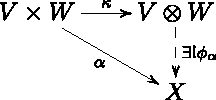
\includegraphics[width=0.3\textwidth]{Dateien/Tensor1.pdf}
\end{center}
wobei $V\otimes W$ der Tensorproduktraum ist. Diese Definition hat folgende Vorteile: \\
\begin{enumerate}
    \item Jeder bilinearen Abbildung $\alpha$ kann genau eine Lineare Abbildung $\Phi_\alpha$ zugeordent werden.
    \item Der Tensorproduktraum ist bis auf Isomorphie eindeutig. Seien nämlich zwei Räume $V\otimes W$ und $V\Tilde{\otimes}W$ gegeben, dann gilt für $X=V\Tilde{\otimes}W$:
\begin{center}
    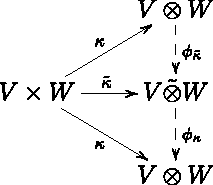
\includegraphics[width=0.28\textwidth]{Dateien/Tensor2.pdf}
\end{center}
und damit $$\Phi_\kappa \circ \Phi_{\Tilde{\kappa}}=Id_{V\Tilde{\otimes}W} \quad \Phi_{\Tilde{\kappa}} \circ \Phi_\kappa  =Id_{V\otimes W}$$
Die Abbildungen $\Phi_\kappa$, $\Phi_{\Tilde{\kappa}}$ sind also gegenseitige Umkehrabbildungen und damit Bijektiv!
\item Das Tensorprodukt existiert! Seien dazu $V$ und $W$ Vektorräume mit den Basen $b_i$ und $b_j$ und:
$$\mathcal{V}(V\times W)=\{ T: V\times W \rightarrow \mathbb{K}, T\neq 0 \}$$
Eine Basis von $\mathcal{V}(V\times W)$ ist dann gegeben durch:
$$\delta_{(b_i, b_j)}(V,W)=\begin{cases}
    1 & \mbox{ wenn $v=b_i$ und $w=b_j$} \\
    0 & \mbox{ sonst}
\end{cases}$$
Wir schreiben nun:
$$\alpha(V,W) = \alpha(\sum_i \lambda_ib^i, \sum_j \mu_jb^{,j})=\sum_{i,j} T_{ij}\alpha(b^i, b^{,j})$$
$$\kappa(V, W)= \kappa(\sum_i \lambda_ib^i, \sum_j \mu_jb^{,j})=\sum_{i,j} T_{ij}\delta_{(b^i, b^{,j})}$$
$$\Phi_\alpha(T)=\Phi_\alpha(\sum_{i,j} T_{ij}\delta_{(b^i, b^{,j})})=\sum_{i,j}T_{ij}\alpha(b^i, b^{,j})$$
Bildlich passiert also folgendes:
\begin{center}
    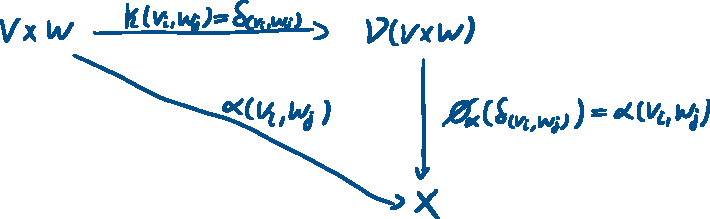
\includegraphics[width=0.7\textwidth]{Dateien/Tensor3.pdf}
\end{center}
Diese Definitionen erfüllen alle benötigten Eigenschaften. Allegemin schreibt man:
$$\kappa(b^i, b^{,j})=b^i\otimes b^{,j}$$
\end{enumerate}
\end{Def}

\begin{Satz}{Regeln}{Eigenschaften des Tensorprodukts}
\begin{enumerate}
    \item Für endlichdimensionale Vektorräume gilt
    $$dim_{\mathbb{K}}V\otimes W = dim_{\mathbb{K}} V \cdot dim_{\mathbb{K}} W$$
    \item Sind $V,W$ Hilberträume, lässt sich das Skalarprodukt erweitern:
    $$\braket{v\otimes w, v'\otimes w'}=\braket{v,v'}\cdot \braket{w, w'} \quad \forall v,v'\in V\quad w,w'\in W$$
    \item Es sei $$\alpha: V\rightarrow V' \quad \beta:W\rightarrow W' \quad \alpha\otimes\beta: V\otimes W \rightarrow V'\otimes W'$$
    dann gilt:
    $$(\alpha\otimes\beta)(V\otimes W)=\alpha(V)\otimes \beta(W)$$
    \item Das Tensorprodukt ist bilinear:
    $$(\lambda_1\Phi_1+\lambda_2\Phi_2)\otimes \Psi = \lambda_1\Phi_1 \otimes \Psi + \lambda_2\Phi_2 \otimes \Psi$$
    $$\Phi\otimes (\lambda_1\Psi_1+ \lambda_2\Psi_2) = \lambda_1\Phi \otimes \Psi_1 + \lambda_2\Phi \otimes \Psi_2$$
    \item Elemente der Form
    $$V\otimes W=\kappa(V,W)$$
    heißen Tensorprodukte oder reine Tensoren. Es gibt aber auch Elemente, die die Eigenschaft nicht erfüllen, wie zum Beispiel:
    $$b^1\otimes b^{,1}+b^2\otimes b^{,2}$$
\end{enumerate}
\end{Satz}
\begin{Def}{Transformation von Tensoren}
    Wir betrachten die Vektorräume $V,V'$ mit Basen $e_i$ und $e_i'$ sowie $W, W'$ mit Basen $f_i, f_i'$. Für lineare Abbildungen $\Phi$ und $\Psi$ gilt:
    $$\Phi(e_i)=\sum_k a^k _i e_k' \quad \Psi(f_i)=\sum_l a^k _e e_k'$$
    und daraus folgt:
    $$(\Phi \otimes \Psi)(x^{ij}e_i\otimes f_j) =x^{ij}a^k_i b^l_j e_k'\otimes f_l'$$
    obere Indizes werden kovariant transformiert
    $$x^{ij}\mapsto x^{ij}a^k_ib^l_j$$
\end{Def}

\begin{Def}{$k$-fache äußere Produkt}
Das \red{$k$-fache äußere Produkt (Dachprodukt)} eines $\mathbb{K}$-Vektorraums $V$ ist ein Vektorraum $\Lambda^k(V)$, zusammen mit einer $k$-multilinearen alternierenden Abbildung $\wedge: V\times \dots \times V \rightarrow \Lambda^kV$, so dass es für jede $k$-lineare alternierende Abbildung $\alpha: V^k\rightarrow W$ genau eine lineare Abbildung $\Phi_\alpha:\Lambda^kV\rightarrow W$ gibt, so dass das Diagramm.
\begin{center}
    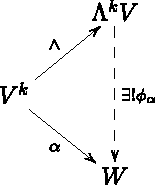
\includegraphics[width=0.28\textwidth]{Dateien/Tensor4.pdf}
\end{center}
kommutiert.    
\end{Def}
Besonders die letzte Definition ist sehr wichtig für spätere Kapitel.
\newpage
\begin{Beispiel}{Einfaches Tensorprodukt von \href{https://www.math3ma.com/blog/the-tensor-product-demystified}{math3ma.com}}
    Seien $V\subseteq \R^3$ und $W\subseteq \R^2$ und wir suchen uns zwei Vektoren aus.
    $$\vec{v}=\begin{pmatrix}
        1 \\
        2 \\
        3 \\
    \end{pmatrix} \qquad \vec{w}=\begin{pmatrix}
        4 \\
        5 \\
    \end{pmatrix}$$
    Wie können wir aus diesen zwei Vektoren einen neuen erstellen? \\
    \begin{enumerate}
        \item mit der Direkten Summe
        \blue{$$\begin{pmatrix}
        1 \\
        2 \\
        3 \\
    \end{pmatrix} \oplus\begin{pmatrix}
        4 \\
        5 \\
    \end{pmatrix} = \begin{pmatrix}
        1 \\
        2\\
        3\\
        4\\
        5\\
    \end{pmatrix}$$
    $$dim(\R^3\oplus \R^2)=dim(\R^3)+dim(\R^2)=5$$}
    \item mit dem Tensorprodukt
    \blue{$$\begin{pmatrix}
        1 \\
        2 \\
        3 \\
    \end{pmatrix} \otimes\begin{pmatrix}
        4 \\
        5 \\
    \end{pmatrix} = \begin{pmatrix}
        1\cdot 4 \\
        1\cdot 5\\
        2\cdot 4\\
        2\cdot 5\\
        3\cdot 4\\
        3\cdot 5
    \end{pmatrix}=\begin{pmatrix}
        4 \\
        5\\
        8\\
        10\\
        12\\
        15
    \end{pmatrix}$$
    $$dim(\R^3\otimes \R^2)=dim(\R^3)\cdot dim(\R^2)=6$$}
    \end{enumerate}
    Das Tensorprodukt ist wie eine erwachsene Version der Multiplikation. Die Basisvektoren von unseren Tensorprodukt sind auch Tensorprodukte der Basisvektoren der jeweiligen Vektorräumen
    $$\begin{pmatrix}
        4 \\
        5\\
        8\\
        10\\
        12\\
        15
    \end{pmatrix}= 4(e_1\otimes e_1) + 5(e_1\otimes e_2)+8(e_2\otimes e_1) + 10(e_2\otimes e_2) + 12(e_3\otimes e_1) + 15(e_3\otimes e_2)$$
\end{Beispiel}
Guckt euch gerne noch die Website an, weil math3ma Tensoren super erklärt.
\begin{Beispiel}{Tensorprodukte in der Quantenmechanik}
    Der Spinzustand $\ket{\chi}$ lebt in Spinraum $H_s$ und der Ortszustand $\ket{\psi}$ im Ortsraum $H_r$. Der Gesamtzustand lebt im Tensorproduktraum
    $$\ket{\psi}\otimes\ket{\chi} \in H_r\otimes H_s$$
    Auch Vielteilchenzustände sind Tensorprodukte von Einteilchenzuständen.
\end{Beispiel}
\begin{Beispiel}{Nützliche Tensorwerkzeuge aus den Präsenzaufgaben}
\begin{enumerate}
    \item Jedes Element von $V\otimes W$ lässt sich schreiben als
    \blue{$$v_1\otimes w_1 + v_2\otimes w_2 \quad \mbox{mit $v_1,v_2\in V$ und $w_1,w_2\in W$}$$}
    \item Ein \red{reiner Tensor} hat immer die Form
    \blue{$$a\otimes b \quad \mbox{$a\in V$ und $b\in W$}$$}
    \item Wie finden wir ein Element von $\R^3 \otimes \R^2$, dass nicht als ein reiner Tensor dargestellt werden kann?\\
    \blue{Am besten wir stellen uns eine Matrix auf und versuchen dann so eine zu finden, deren Rang mindestens 2 ist
    $$
      ^{e_1}_{e_2}\begin{cases}
          \overbrace{\begin{pmatrix}
     1 & 0 & 0\\
     0 & 1 & 0
  \end{pmatrix}}^{e_1 \quad e_2 \quad e_3}
      \end{cases}$$
      Und tatsächlich haben wir hier schon so eine Matrix gefunden und unser Tensor ist $$e_1\otimes e_1+e_2\otimes e_2$$}
      \item Zeige, dass $x\in V\otimes V$ ungleich Null ist:
      \blue{$$x=\begin{pmatrix}
          3 \\ 0
      \end{pmatrix}\otimes \begin{pmatrix}
          2 \\ 3
      \end{pmatrix}+\begin{pmatrix}
          0 \\ 9
      \end{pmatrix}\otimes \begin{pmatrix}
          1 \\ 0
      \end{pmatrix}=\begin{pmatrix}
          6 \\ 9 \\ 0 \\ 0
      \end{pmatrix}+ \begin{pmatrix}
          0 \\ 0 \\ 9 \\ 0
      \end{pmatrix}=\begin{pmatrix}
          6 \\ 9 \\ 9 \\ 0
      \end{pmatrix}\neq 0$$}
      \item Sei $y\in \Lambda^2 V$. Zeige, dass $y=0$:
      
      \blue{$$y=\begin{pmatrix}
          3 \\ 0
      \end{pmatrix}\wedge \begin{pmatrix}
          2 \\ 3
      \end{pmatrix}+\begin{pmatrix}
          0 \\ 9
      \end{pmatrix}\wedge \begin{pmatrix}
          1 \\ 0
      \end{pmatrix}$$
      Hier ist vorerst die Definition des} \red{2D-Dachproduktes} \blue{wichtig}. 
      \red{$$a\wedge b = \det \begin{pmatrix}
          a_1 & a_2 \\
          b_1 & b_2
      \end{pmatrix}= a_1b_2-a_2b_1$$}
      \blue{$$y=9-9=0$$}
\end{enumerate}
\end{Beispiel}


\end{document}